\documentclass[journal,a4paper,onecolumn]{IEEEtran}

\usepackage{graphicx}
\usepackage{url}
\usepackage{amsmath}
\usepackage{booktabs}
\usepackage{longtable}
\usepackage{array}
\usepackage{enumitem}
\usepackage{xcolor}
\usepackage{hyperref}
\usepackage{float}
\usepackage[UTF8,scheme=plain]{ctex}

\graphicspath{{diagrams/}{assets/media/}}
\hypersetup{colorlinks=true,linkcolor=blue,urlcolor=blue,citecolor=blue}
\setlength{\LTpre}{4pt}
\setlength{\LTpost}{4pt}
\newcommand{\HRule}{\rule{\linewidth}{0.5mm}}
\newcommand{\req}[1]{\textbf{#1}}
\newcommand{\statusimpl}{\textbf{DDL 已实现}}
\newcommand{\statusapp}{\textbf{应用层责任}}
\newcommand{\statusgate}{\textbf{实施门禁}}

\begin{document}
\begin{titlepage}
\center
~\\[0.5cm]
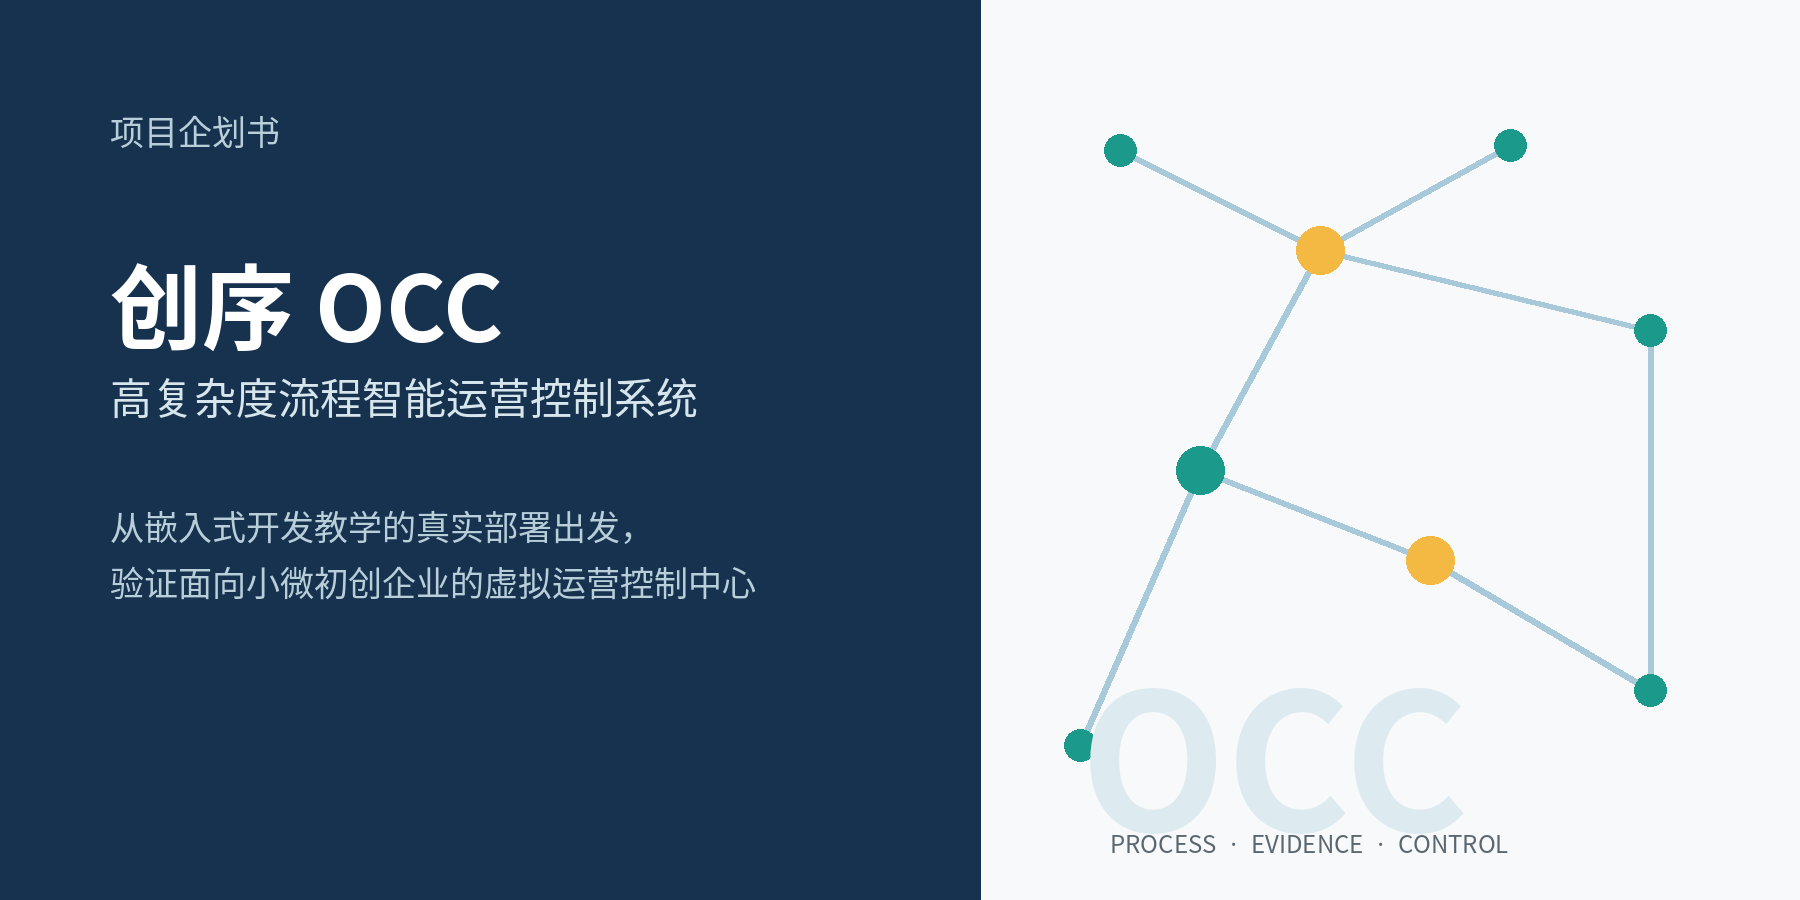
\includegraphics[width=0.88\textwidth]{image1.png}\\[1.0cm]
\HRule \\[0.6cm]
{\huge\bfseries 创序 OCC 软件规格与数据库设计}\\[0.3cm]
{\Large Software Specification and Database Design}\\[0.6cm]
\HRule \\[1.2cm]
\textsc{\Large 文档语言：中文}\\[0.5cm]
\textsc{\Large 基线：16 周 MVP 与后续领域扩展}\\[1.2cm]
\begin{minipage}{0.42\textwidth}
\begin{flushleft}\large
\emph{系统：}\\
创序 OCC
\end{flushleft}
\end{minipage}
\begin{minipage}{0.42\textwidth}
\begin{flushright}\large
\emph{文档版本：}\\
1.0
\end{flushright}
\end{minipage}\\[1.2cm]
{\large 编制日期：2026-07-28}\\[0.5cm]
{\large 状态：设计基线 / 实施前规格}\\[1cm]
\vfill
\end{titlepage}

\title{创序 OCC：软件规格与数据库设计}
\author{Innorder OCC Project Documentation}
\maketitle

\begin{abstract}
本文档以项目企划书、技术选型与架构设计、数据库表设计、八个 PostgreSQL/Flyway 迁移及其契约测试为事实来源，定义创序 OCC 的软件需求、架构边界、领域模型、关键事务、安全与治理、非功能要求和数据库物理设计。系统采用“确定性流程控制面 + 概率智能面”：Flowable 与 OCC Core 负责可验证的状态、权限、证据和审计；AI Service 负责理解、检索、规划、核验和风险建议，但不得直接推进关键流程事实。本文同时区分已经由 DDL 强制保证的约束、必须由应用层实现的规则，以及上线前仍需验证的门禁。
\end{abstract}

\tableofcontents
\clearpage

\section{文档目的与依据}
\subsection{目的}
本规格用于指导 MVP 实现、数据库评审、接口设计、测试验收和私有部署交付。它不是营销说明，也不把规划中的组件描述为已完成代码。当前仓库包含完整数据库迁移与测试，但不包含 Electron、OCC Core、AI Service、OPA bundle 或 Docker Compose 的应用实现。

\subsection{事实来源与优先级}
\begin{longtable}{p{0.27\textwidth}p{0.18\textwidth}p{0.47\textwidth}}
\toprule
来源 & 状态 & 本文使用方式 \\
\midrule
\endhead
项目企划书 V1.0 & 产品愿景 & 定义首个教学场景、用户价值、16 周路线、指标和风险边界。\\
技术选型与架构设计 & 已确认设计 & 定义技术栈、服务边界、事务与事件模型、降级、安全和性能基线。\\
数据库表设计 & 已确认设计 & 定义 schema 划分、数据语义、授权模型、AI/RAG 模型和治理原则。\\
V001--V008 SQL 迁移 & 可执行实现 & 数据库对象、字段、约束、触发器、索引和分区的最终依据；与设计文档冲突时以 DDL 描述“现状”。\\
数据库测试与 README & 验证证据 & 说明已覆盖的契约和仍未在真实 PostgreSQL/pgvector 上验证的内容。\\
\bottomrule
\end{longtable}

\subsection{术语}
\textbf{OCC} 指运营控制中心；\textbf{领域包}是可发布的 BPMN、DMN、表单、角色、证据规则、风险规则、知识源和 UI 元数据集合；\textbf{业务事实}是能改变流程、任务、证据或审核结果的权威状态；\textbf{建议}是 AI 输出，必须经规则、证据或人工批准后才能影响关键业务事实；\textbf{共享授权实体}是登记在 \texttt{authz.entity} 中并参与统一关系图与 OPA 决策的主体或资源。

\section{产品范围}
\subsection{目标}
\begin{enumerate}[leftmargin=*]
\item 将复杂领域流程表达为标准 BPMN、确定性规则、版本化表单和证据要求，并直接执行。
\item 为参与者维护当前可执行任务、阻塞原因、等待期任务和风险状态。
\item 让关键状态变化具备身份、权限、证据、版本、原因和审计链。
\item 以每客户独立实例私有部署，兼容客户 OIDC、对象存储、Kafka、Redis 和模型服务。
\item 通过版本化领域包扩展教学之外的领域，不复制核心服务。
\item 在 AI、Kafka 或 Redis 故障时维持核心流程正确性。
\end{enumerate}

\subsection{首版非目标}
首版不实现单实例多租户、完整离线写入、事件溯源、自研 BPMN 引擎、Kubernetes/服务网格、自动提交政府或第三方不可逆操作，也不允许 AI 自动决定最终成绩或高责任合规结论。首版不构建通用行业合规库、供应商撮合网络或五个独立 Agent 微服务。

\subsection{角色与主要用例}
\begin{longtable}{p{0.18\textwidth}p{0.35\textwidth}p{0.39\textwidth}}
\toprule
角色 & 主要目标 & 核心用例 \\
\midrule
\endhead
参与者/学生 & 明确下一步并减少无效等待 & 查看今日任务与路线；提交证据；查看阻塞；预约资源；获得带来源辅导。\\
流程负责人/教师 & 只处理需要判断的事项 & 班级/项目雷达；审核证据；退回或附加条件；处理风险；授权例外；复盘瓶颈。\\
领域建模者 & 维护可发布流程资产 & 编辑 BPMN/DMN/表单；配置证据、风险和角色；校验、比较、发布领域包。\\
管理员 & 维护安全与运行基线 & 账号/OIDC 映射；关系与策略；模型供应商；保留策略；部署与审计。\\
资源管理员 & 管理稀缺资源 & 管理设备、场地、人员时段、容量和预约冲突。\\
AI Service & 产生受治理的建议 & 消费事件；授权检索；调用白名单工具；记录运行、引用和建议。\\
\bottomrule
\end{longtable}

\begin{figure}[H]
\centering
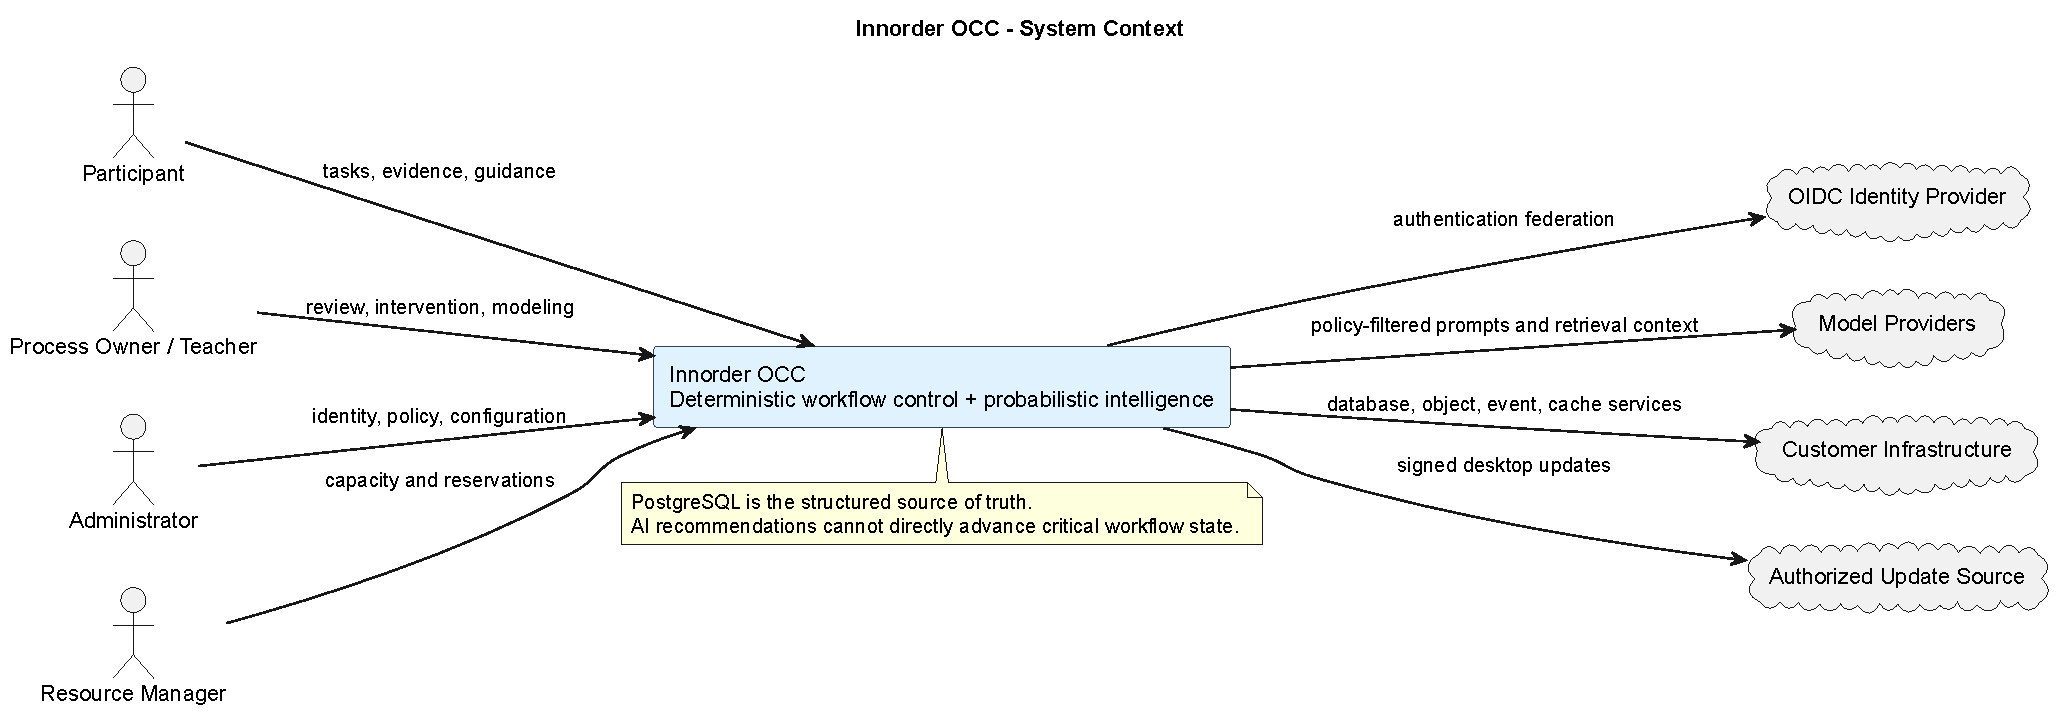
\includegraphics[width=0.98\textwidth]{01-system-context.pdf}
\caption{系统上下文：用户、客户基础设施和外部服务边界。}
\label{fig:context}
\end{figure}

\section{架构规格}
\subsection{总体架构}
系统采用 Electron 桌面端、Kotlin/Spring Boot 模块化单体 Core、Node.js/LangChain.js AI Service，以及 PostgreSQL、Flowable、OPA、Kafka、Redis 和 S3 兼容对象存储。所有组件按客户独立部署。Electron 只访问 OCC 领域 API；AI 只访问受限 Core API、授权事件及 AI 自有数据库对象；任何消费者不得直接推进 Flowable 关键状态。

\begin{figure}[H]
\centering
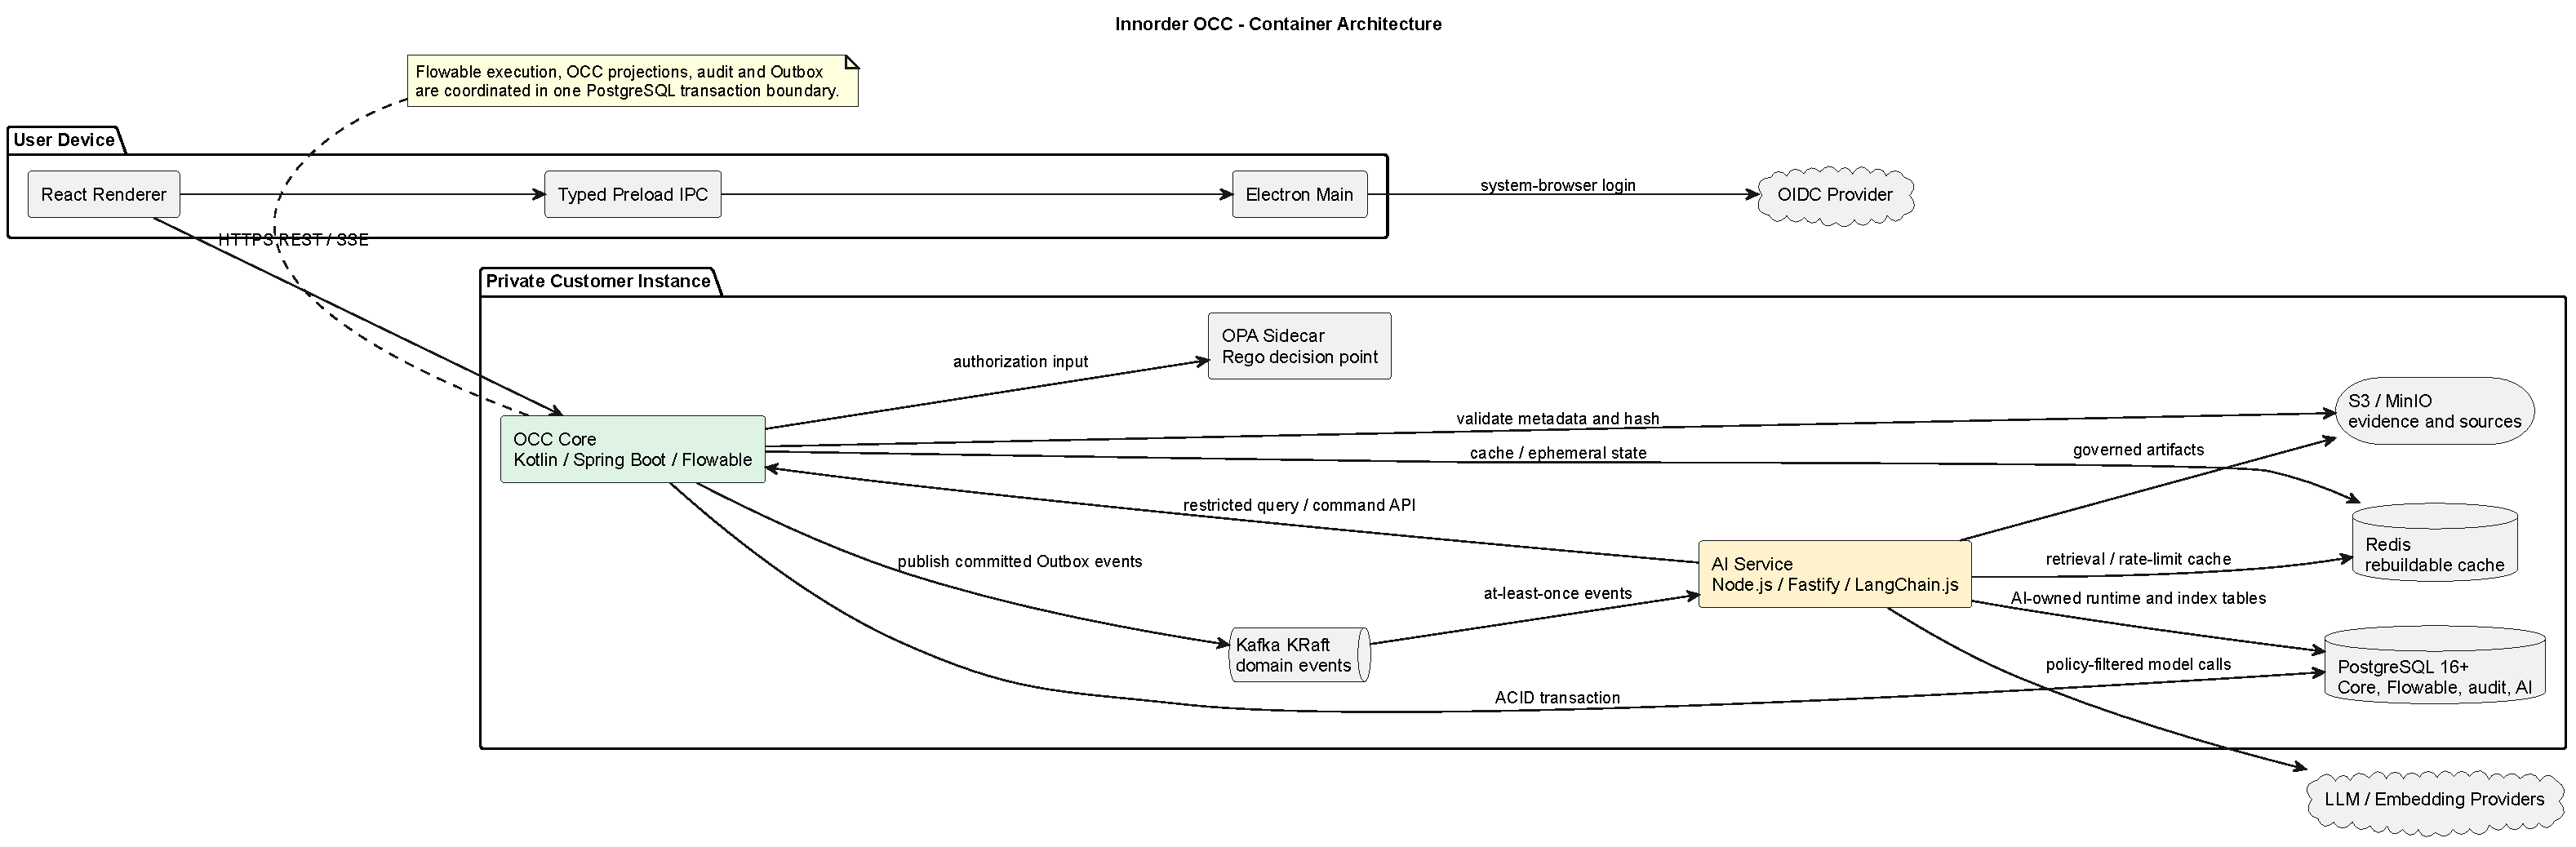
\includegraphics[width=\textwidth]{02-container-architecture.pdf}
\caption{容器架构与同步、异步通信边界。}
\label{fig:containers}
\end{figure}

\subsection{架构不变量}
\begin{enumerate}[leftmargin=*]
\item PostgreSQL 是结构化业务事实的唯一权威来源；Kafka 不是主存储，Redis 数据必须可丢失和重建。
\item Core 在同一事务中协调 Flowable、OCC 投影、授权关系、审计和 Outbox。
\item 对象上传只有经 Core 校验存在性、类型、大小和 SHA-256，并提交证据元数据后才有效。
\item OPA 是无状态决策面；PostgreSQL 保存身份、直接关系、授权属性和已发布策略版本。
\item 任何适用 DENY 覆盖 ALLOW；无匹配、OPA 错误或 revision 不一致时默认拒绝。
\item AI 输出始终是建议或人工队列项，不能绕过 BPMN、DMN、证据要求和人工闸门。
\item 领域包不得携带任意脚本、DDL 或密钥；服务任务只能引用预注册能力标识。
\end{enumerate}

\subsection{Core 模块边界}
\begin{figure}[H]
\centering
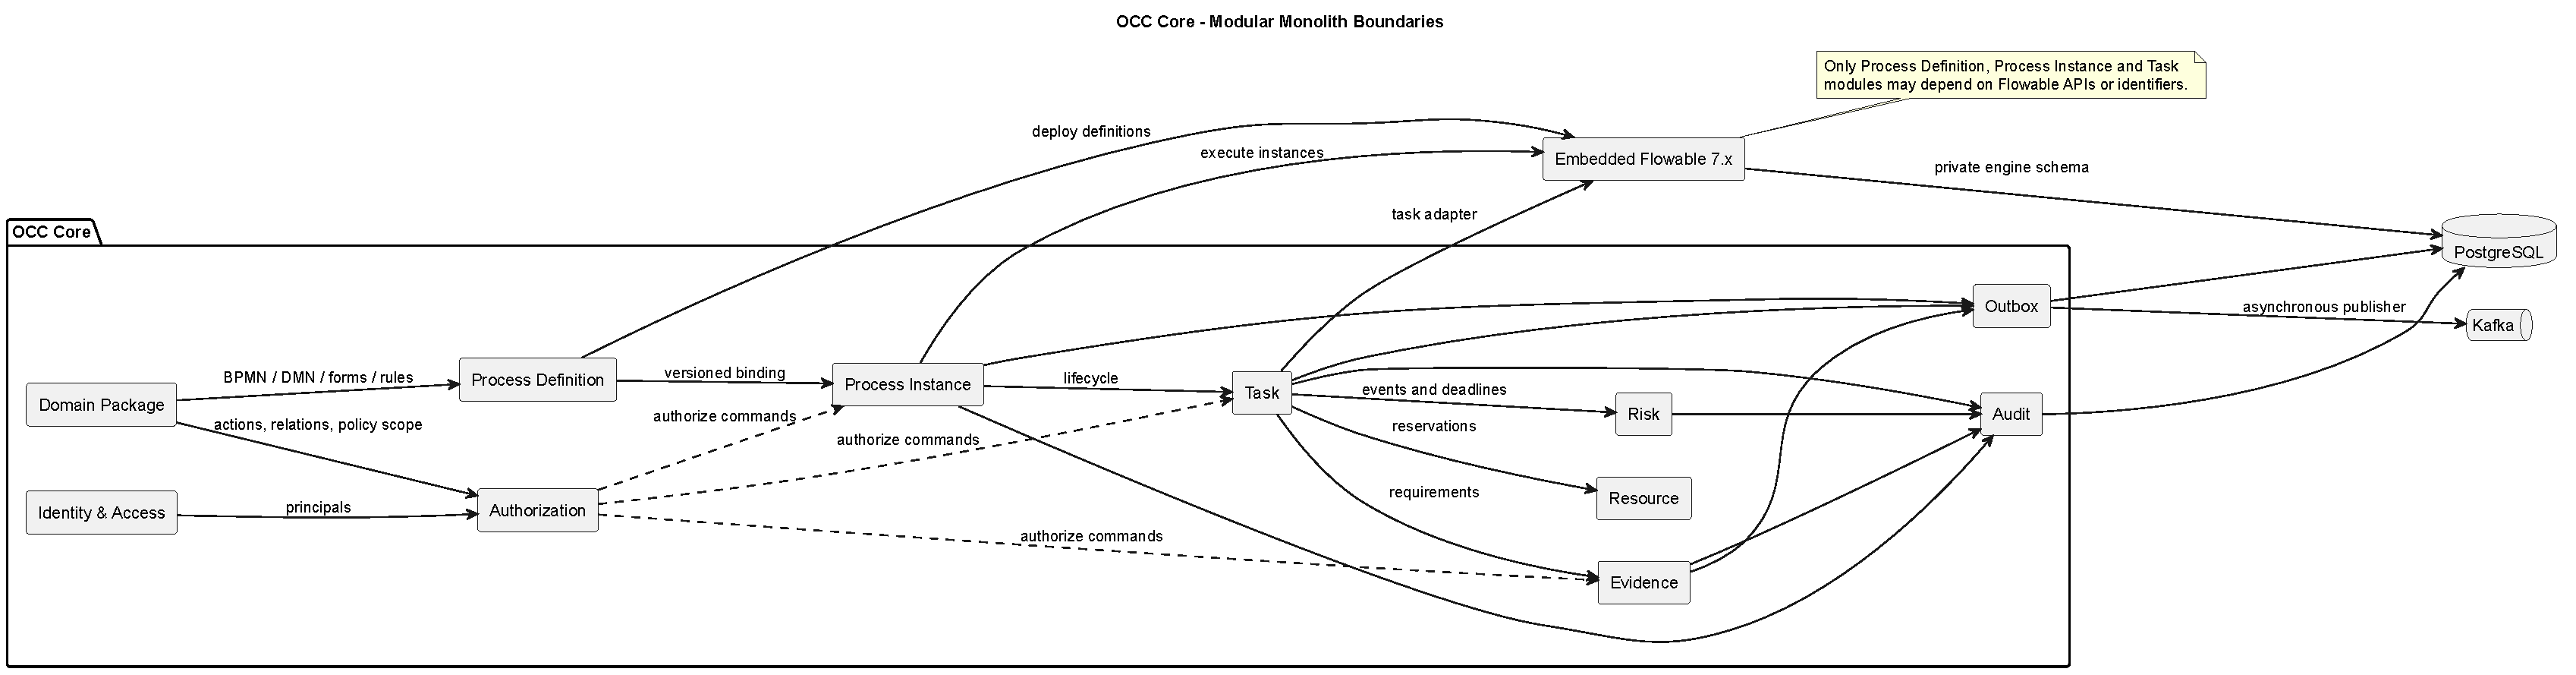
\includegraphics[width=0.94\textwidth]{03-core-modules.pdf}
\caption{OCC Core 模块及 Flowable 封装边界。}
\label{fig:modules}
\end{figure}

Process Definition、Process Instance 和 Task 是唯一可依赖 Flowable API 或引擎标识的模块。其他模块通过内部领域接口协作，不读取 Flowable 私有表。Identity \& Access 管理认证主体；Authorization 构造事务快照并调用 OPA；Domain Package 管理版本化资产；Evidence、Risk、Resource、Audit 和 Outbox 分别维护证据、干预、预约、不可变追踪和事件发布。

\section{功能需求}
\subsection{身份与授权}
\begin{longtable}{p{0.12\textwidth}p{0.66\textwidth}p{0.14\textwidth}}
\toprule
编号 & 需求 & 验证层 \\
\midrule
\endhead
\req{FR-IAM-01} & 系统应支持内置用户账号与 OIDC 外部身份映射；组和角色不可直接登录。 & Core/集成测试\\
\req{FR-IAM-02} & 所有可授权主体和资源应登记为统一实体，并使用稳定业务键、类型版本和乐观锁版本。 & \statusimpl\\
\req{FR-AZ-01} & 写命令应在事务内锁定 authorization revision，读取直接关系和 active policy release 后调用本地 OPA。 & Core/并发测试\\
\req{FR-AZ-02} & 关系定义应校验主体类型、对象类型、基数、有效期、发布状态及可选无环约束。 & \statusimpl\\
\req{FR-AZ-03} & 策略应按 PLATFORM、DOMAIN、CUSTOMER 三层组成原子 release；必须存在平台层，且同时只能有一个 ACTIVE release。 & 部分 DDL + Core\\
\req{FR-AZ-04} & 允许的写决策应与业务审计同事务保存；拒绝决策应在独立追加事务保存。 & Core/集成测试\\
\bottomrule
\end{longtable}

\subsection{领域包与流程}
\begin{longtable}{p{0.12\textwidth}p{0.66\textwidth}p{0.14\textwidth}}
\toprule
编号 & 需求 & 验证层 \\
\midrule
\endhead
\req{FR-DP-01} & 领域包版本应包含 manifest、BPMN/DMN 引用、JSON Schema 表单、动作、关系、证据、风险和知识配置。 & Catalog/API\\
\req{FR-DP-02} & 状态应遵循 DRAFT、VALIDATED、PUBLISHED、DEPRECATED；发布内容应具有 SHA-256 且不可修改。 & \statusimpl\\
\req{FR-DP-03} & 发布前应校验语法、引用、禁用元素、权限、回归场景和运行实例影响。 & \statusapp\\
\req{FR-WF-01} & 每个流程实例应显式绑定 package version 和 Flowable definition binding，新发布不得隐式改变运行实例。 & DDL + Core\\
\req{FR-WF-02} & 命令应使用幂等键和 expectedVersion；重复请求返回原结果，请求哈希冲突或版本冲突返回 409。 & Core/集成测试\\
\req{FR-WF-03} & 任务应支持创建、领取、完成、取消和失败，负责人/候选人/审核人通过关系图表达。 & Core/API\\
\req{FR-WF-04} & Flowable 变更、OCC 投影、审计和 Outbox 应原子提交。 & \statusgate\\
\bottomrule
\end{longtable}

\subsection{证据、风险与资源}
\begin{longtable}{p{0.12\textwidth}p{0.66\textwidth}p{0.14\textwidth}}
\toprule
编号 & 需求 & 验证层 \\
\midrule
\endhead
\req{FR-EV-01} & 客户端应使用短期上传会话直接上传对象存储，Core 校验后才创建不可变证据版本。 & DDL + 集成测试\\
\req{FR-EV-02} & 证据至少绑定任务或业务对象，按 requirement 验证类型、大小、数量和验收条件。 & 部分 DDL + Core\\
\req{FR-EV-03} & 审核应只追加，支持 ACCEPTED、REJECTED、CONDITIONAL，并保存审核人、原因和条件。 & \statusimpl\\
\req{FR-RI-01} & 风险应保存规则、目标、INFO/YELLOW/RED 等级、状态、置信度、原因、期限和处置时间。 & \statusimpl\\
\req{FR-RS-01} & 排他预约不得在同一资源和活动时段重叠；容量型预约应在事务中锁定资源并校验总容量。 & DDL + Core\\
\bottomrule
\end{longtable}

\subsection{AI、RAG 与协作}
\begin{longtable}{p{0.12\textwidth}p{0.66\textwidth}p{0.14\textwidth}}
\toprule
编号 & 需求 & 验证层 \\
\midrule
\endhead
\req{FR-AI-01} & AI Service 应支持规划、辅导、核验、风险和监督职责，共享受控工具、追踪和评测设施。 & AI Service\\
\req{FR-AI-02} & 模型配置应声明能力、数据策略、超时、限流和成本；能力不足时拒绝执行。 & DDL + AI Service\\
\req{FR-AI-03} & 工具调用应使用结构化 schema、白名单 grant、所需 action 和 OPA 决策日志。 & DDL + 契约测试\\
\req{FR-RAG-01} & 检索必须先授权 knowledge document ID，再在候选集合内执行全文、向量和重排。 & AI Service/安全测试\\
\req{FR-RAG-02} & 同时只能有一个 ACTIVE embedding space；新空间达到覆盖率和评测门槛后原子切换。 & 部分 DDL + AI Service\\
\req{FR-AI-04} & 建议应记录运行、目标、payload、置信度、状态和版本化引用；接受建议仍须执行普通授权命令。 & DDL + Core\\
\req{FR-AI-05} & 消息、引用、提示词版本、文档版本和评测数据应可追溯；生成内容应明确标识。 & DDL + UI\\
\bottomrule
\end{longtable}

\section{领域模型与状态}
\begin{figure}[H]
\centering
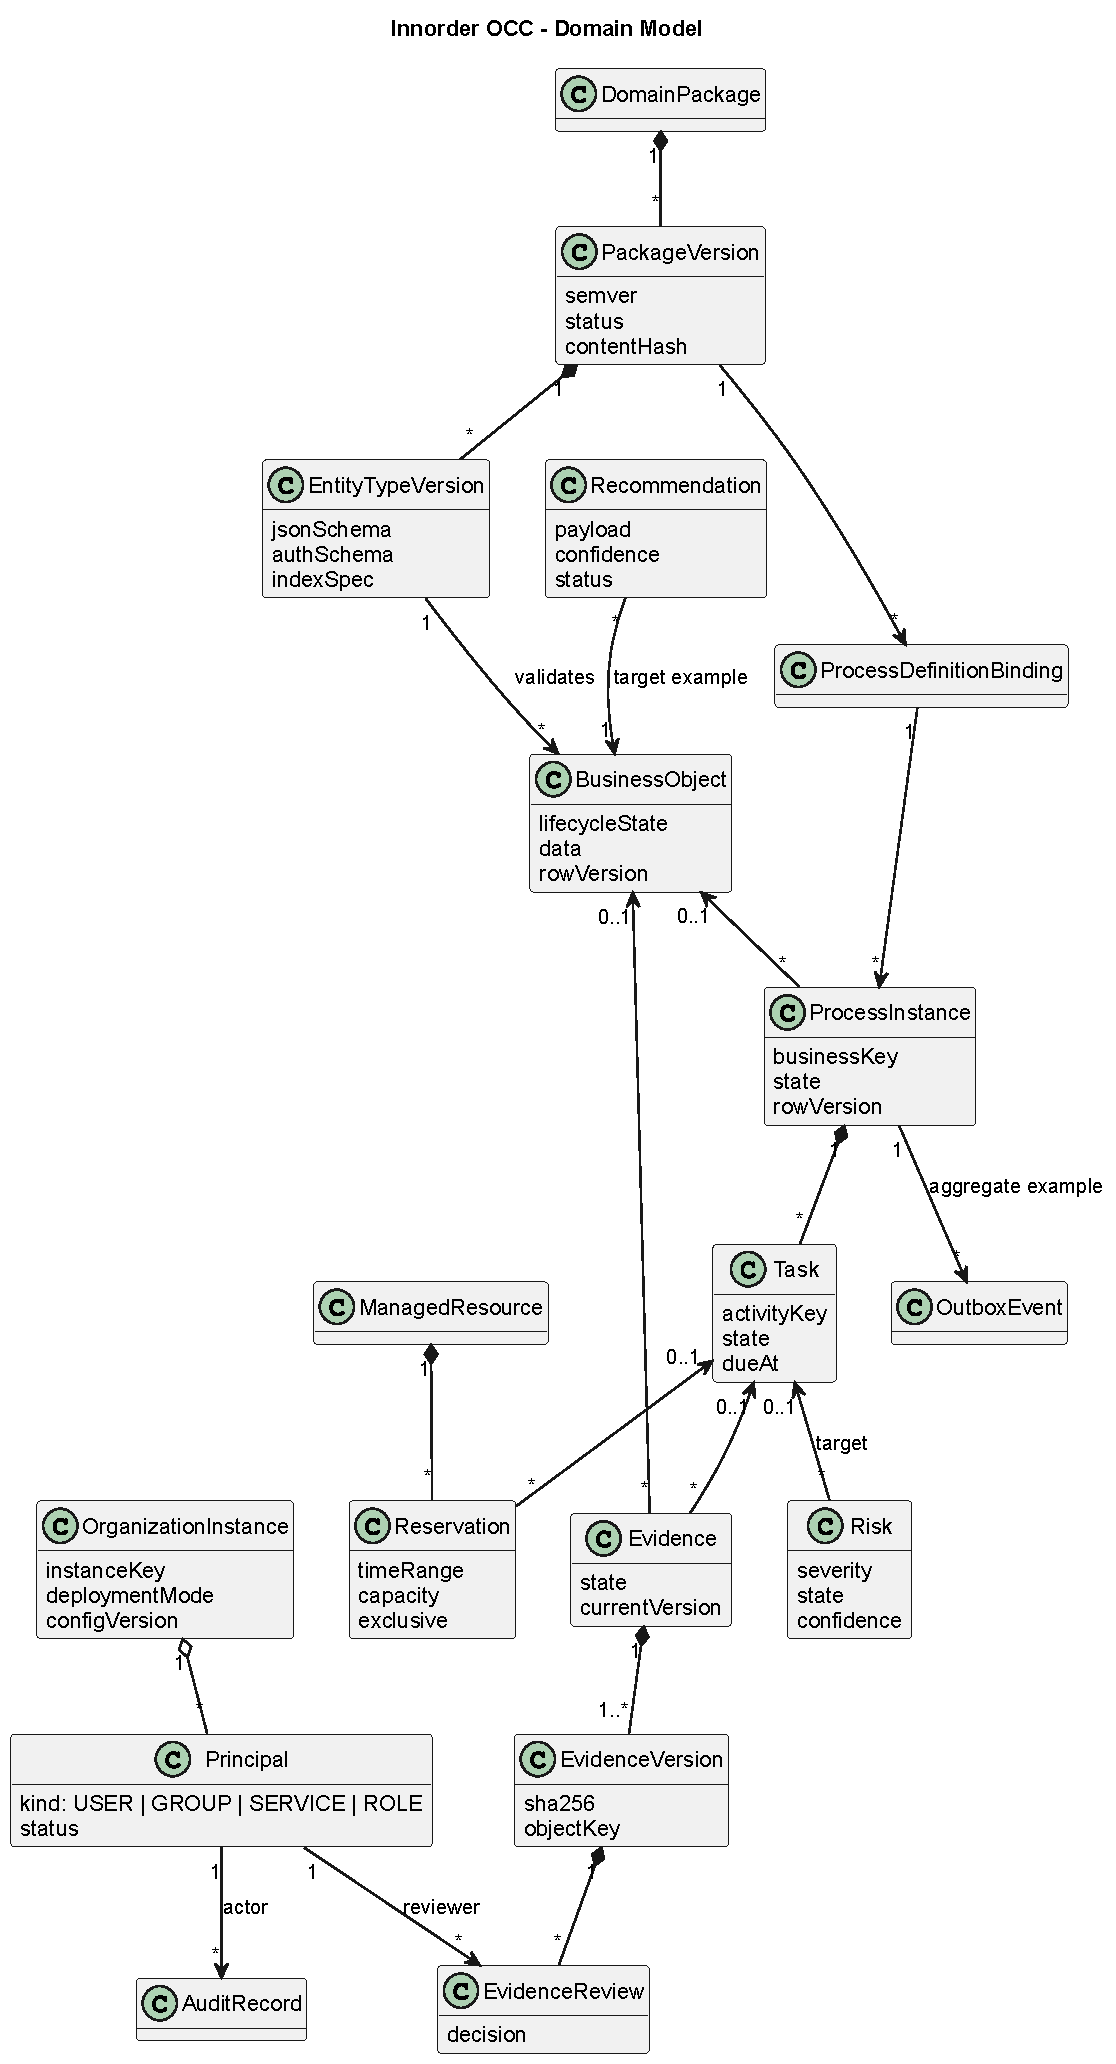
\includegraphics[width=\textwidth,height=0.74\textheight,keepaspectratio]{04-domain-model.pdf}
\caption{稳定领域概念及主要聚合关系。}
\label{fig:domain}
\end{figure}

\subsection{聚合边界}
领域包及其版本化定义构成发布聚合；业务对象是可扩展领域数据聚合；流程实例与任务是 Flowable 状态的 OCC 授权投影；证据由可变头记录、不可变版本和只追加审核组成；风险与预约分别是干预和资源占用聚合；AI run 是执行追踪，recommendation 是可授权且可审核的业务建议。

\subsection{关键生命周期}
\begin{longtable}{p{0.25\textwidth}p{0.60\textwidth}}
\toprule
对象 & 状态及约束 \\
\midrule
\endhead
Package Version & DRAFT $\rightarrow$ VALIDATED $\rightarrow$ PUBLISHED $\rightarrow$ DEPRECATED；发布后内容不可修改。\\
Process Instance & RUNNING/SUSPENDED $\rightarrow$ COMPLETED/CANCELLED/FAILED；终态必须有 ended\_at。\\
Task Projection & CREATED $\rightarrow$ CLAIMED $\rightarrow$ COMPLETED，或 CANCELLED/FAILED；完成必须有 completed\_at。\\
Evidence & PENDING $\rightarrow$ SUBMITTED $\rightarrow$ ACCEPTED/REJECTED，可归档；current\_version 使用延迟 FK。\\
Risk & OPEN $\rightarrow$ ACKNOWLEDGED $\rightarrow$ RESOLVED/DISMISSED；RESOLVED 必须有 resolved\_at。\\
Policy Release & 只能以 STAGED 创建，再转 ACTIVE/RETIRED/FAILED；ACTIVE 全局唯一。\\
Embedding Space & BUILDING $\rightarrow$ ACTIVE $\rightarrow$ RETIRED，或 FAILED；ACTIVE 全局唯一。\\
Recommendation & PROPOSED $\rightarrow$ ACCEPTED/REJECTED/EXPIRED/WITHDRAWN。\\
\bottomrule
\end{longtable}

\section{关键交互与事务语义}
\subsection{授权敏感写命令}
\begin{figure}[H]
\centering
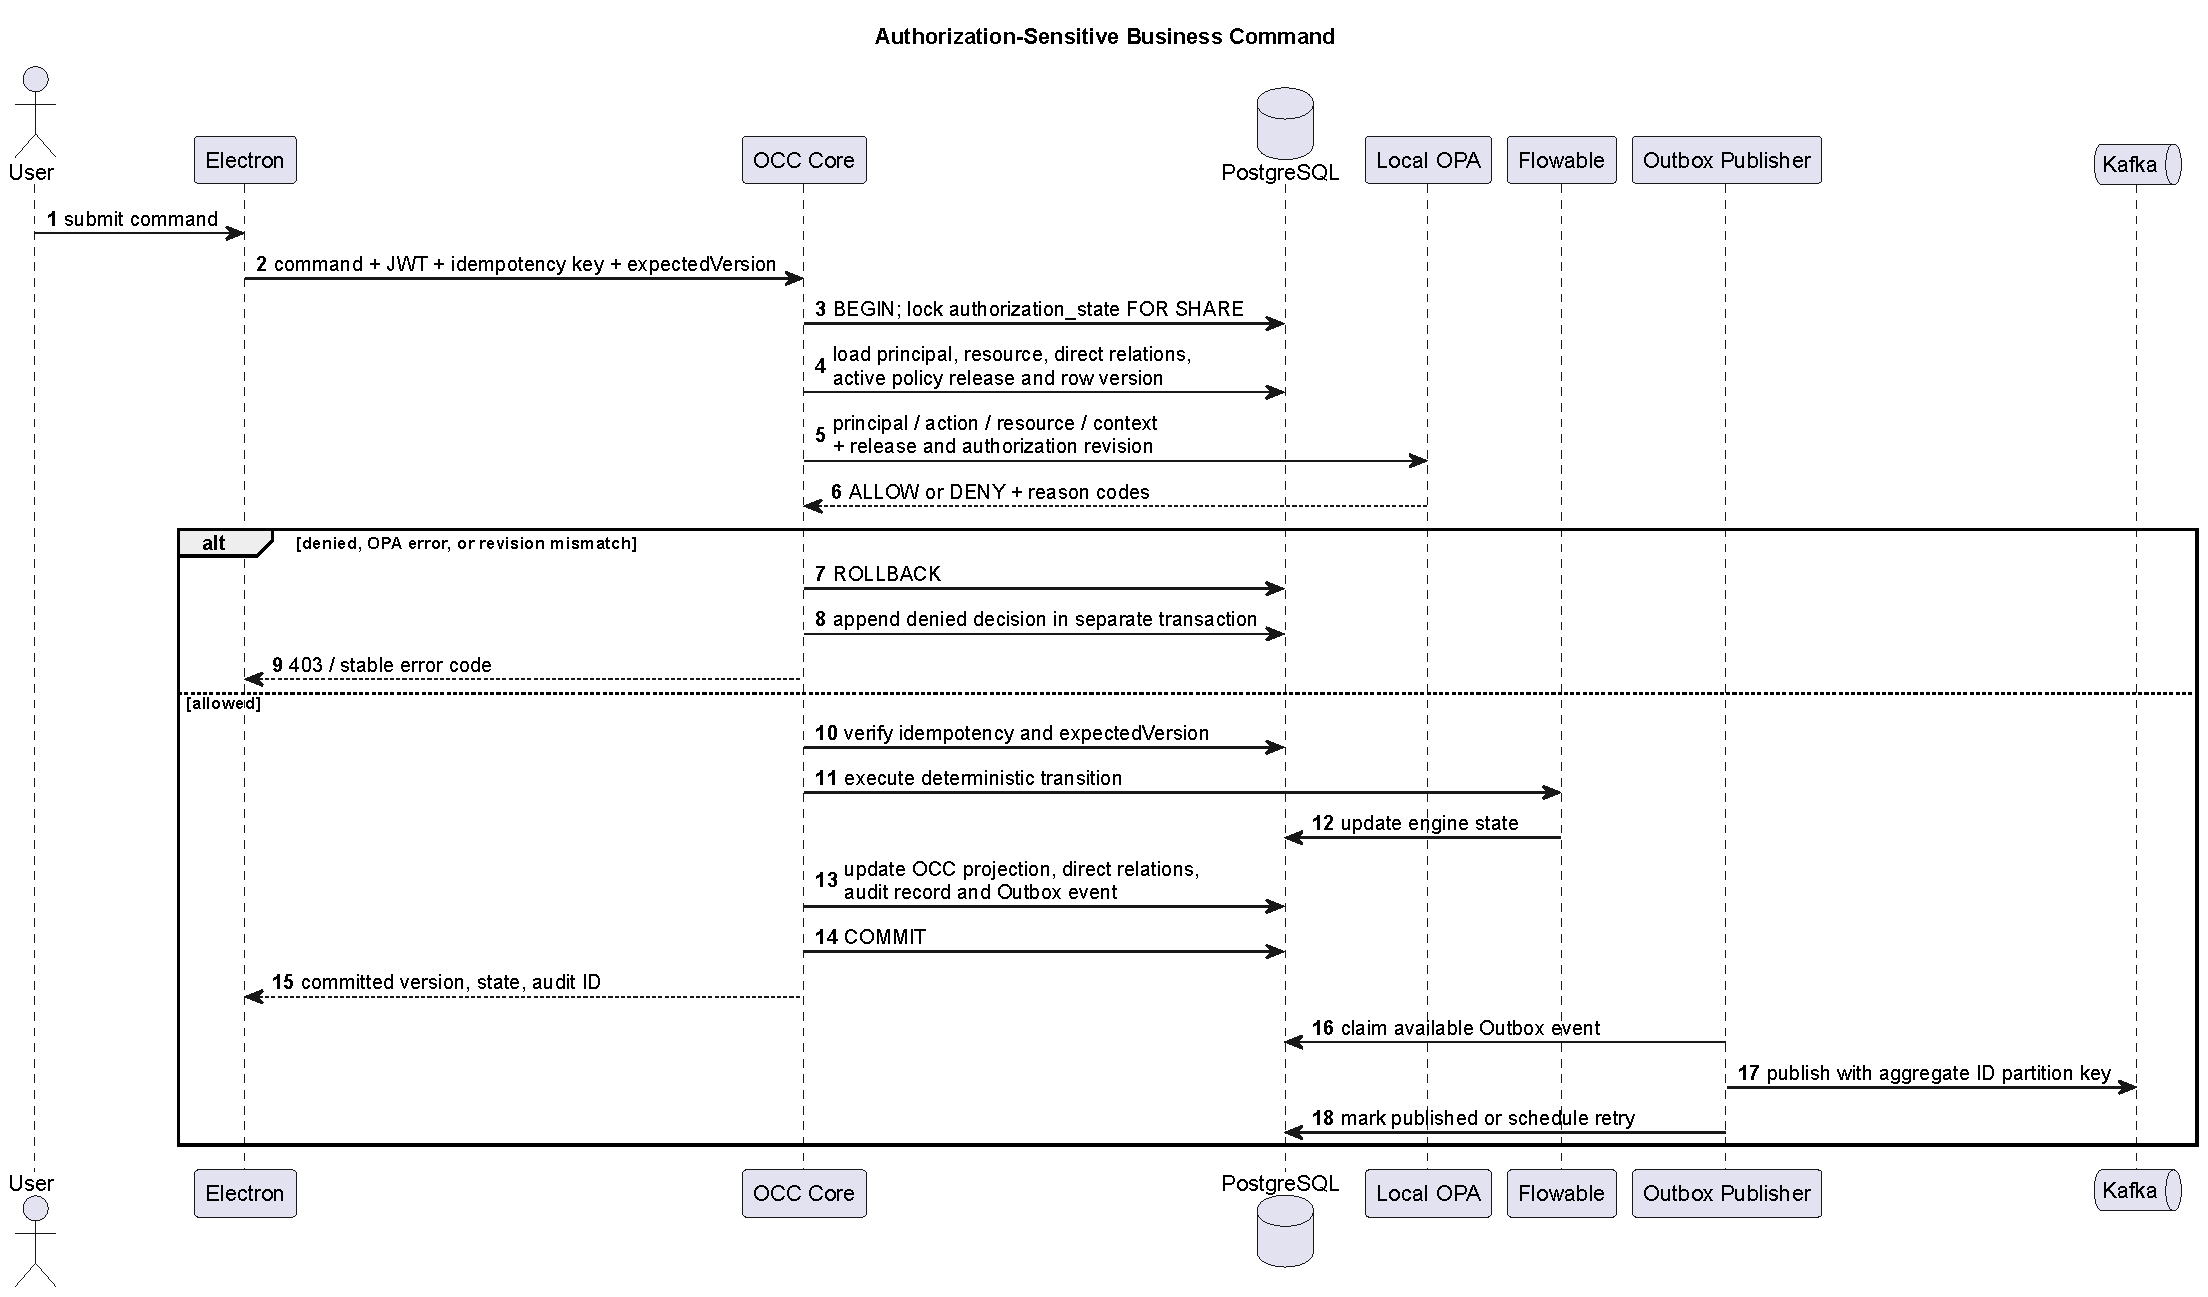
\includegraphics[width=0.90\textwidth]{05-command-transaction-sequence.pdf}
\caption{写命令的授权、乐观锁、Flowable、审计和 Outbox 顺序。}
\label{fig:command}
\end{figure}
普通业务写对 \texttt{authz.authorization\_state} 取共享锁；关系、策略 release、授权属性或实体授权状态变化取排他锁并递增 revision。Core 必须把锁定的 revision 与 policy release 发送给 OPA，并拒绝不一致响应。Kafka 采用至少一次投递；消费者按 event ID 幂等，按 aggregate ID 分区以保持聚合内顺序。

\subsection{证据提交与审核}
\begin{figure}[H]
\centering
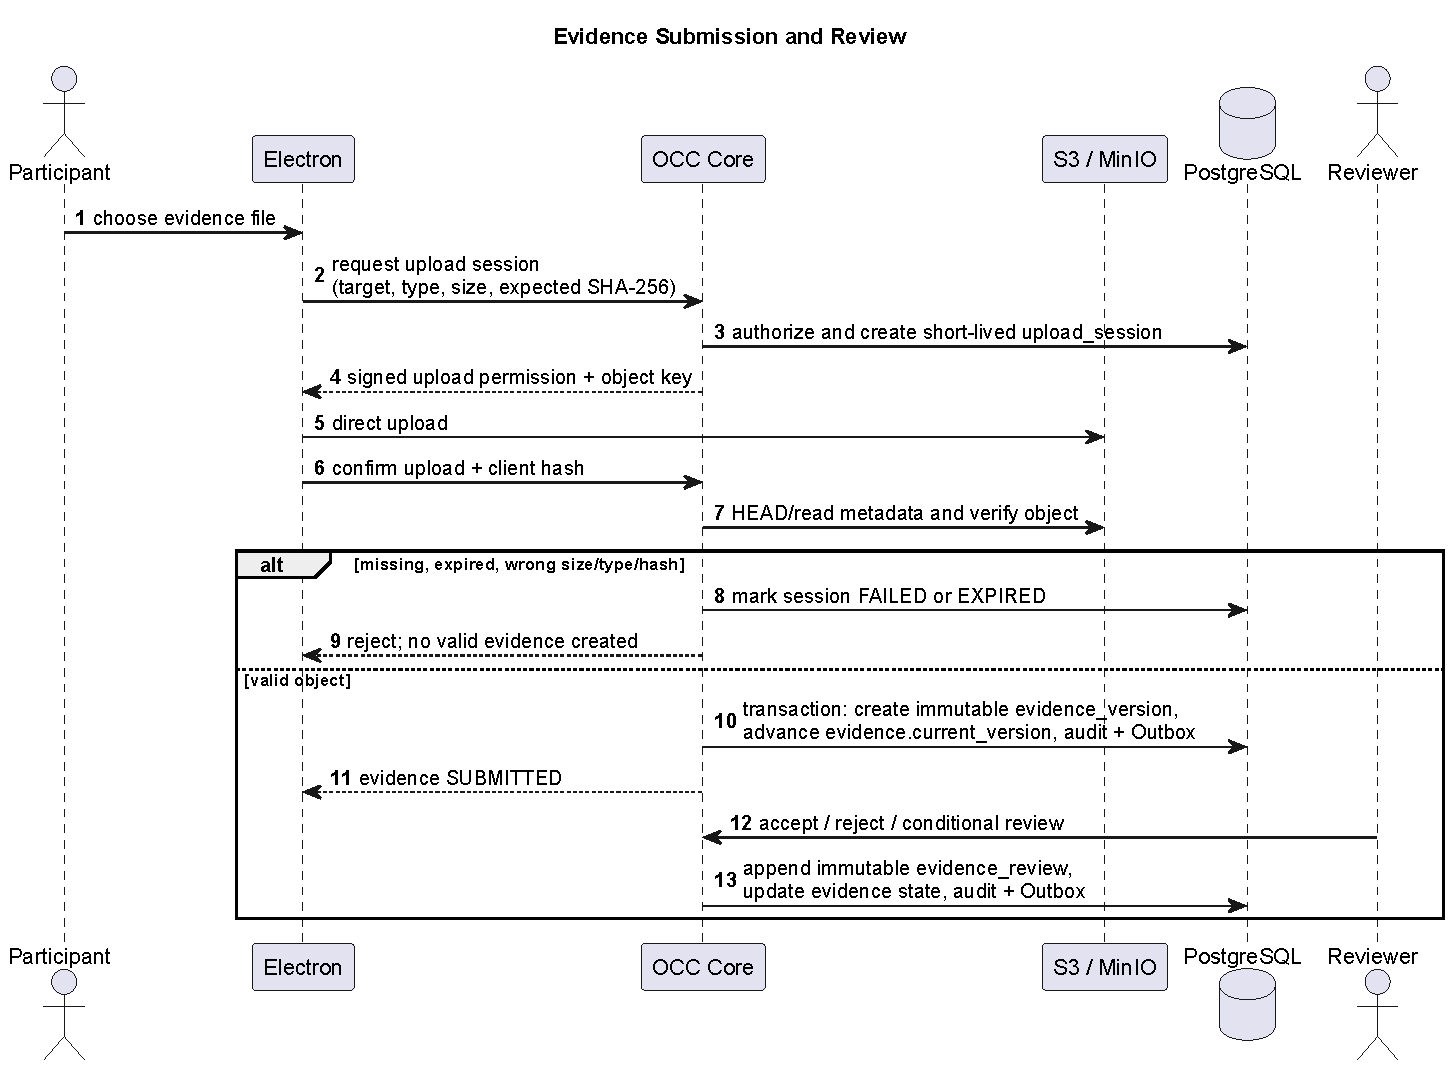
\includegraphics[width=0.88\textwidth]{06-evidence-flow.pdf}
\caption{证据对象从临时上传到有效版本和人工审核的闭环。}
\label{fig:evidence}
\end{figure}

\section{接口与事件契约}
\subsection{同步 API}
REST/OpenAPI 是 Electron、Core 和 AI 的同步契约来源。命令携带 JWT、\texttt{Idempotency-Key}、\texttt{expectedVersion} 和 correlation ID。错误使用 Problem Details，至少包含稳定错误码、可重试属性、correlation ID 和用户可理解说明。查询不得暴露 Flowable 表名、原生实体或内部状态编码。实时通知使用 SSE，可靠通知必须先持久化。

\subsection{事件信封}
Kafka JSON 事件至少包含 event ID、schema version、customer instance ID、aggregate type、aggregate ID、aggregate version、event type、occurred time、correlation ID 和 data classification。兼容性策略必须在 CI 中检查；PostgreSQL 到 Kafka 不承诺 exactly-once。

\section{安全、隐私与治理}
\begin{enumerate}[leftmargin=*]
\item Electron renderer 启用 sandbox、context isolation 和 CSP，关闭 Node integration；令牌仅由主进程通过操作系统安全存储持有。
\item 服务间使用独立身份、TLS 和最小权限数据库账号；密钥只保存 secret reference。
\item 平台 DENY 不可由领域或客户策略覆盖；策略发布需编译、测试、审批、签名、OPA 加载确认和原子切换。
\item auth\_attributes 只允许 auth schema 白名单字段；发送到模型的数据按供应商和分类默认拒绝。
\item 检索内容视为不可信输入，不能改变系统提示、工具 grant、权限或审批规则。
\item 审计、证据版本、策略发布、文档版本和消息通过只追加或不可变约束保护；删除须遵循保留与法律留置。
\item AI 生成内容保留模型、提示词、领域包、知识库、引用、工具调用、成本和追踪信息。
\end{enumerate}

\section{非功能需求}
\subsection{可靠性与降级}
Kafka 不可用时核心事务提交、Outbox 重试；Redis 不可用时回源 PostgreSQL；AI 超时、限流或无有效来源时拒绝建议或升级人工，但不阻塞核心命令；对象存储不可用时不生成有效证据；Core 或 PostgreSQL 不可用时 Electron 仅允许只读缓存，禁止离线写入。

\subsection{性能基线}
在记录硬件、网络和数据规模的代表性私有服务器上，以 100 并发会话验证：缓存命中查询 p95 $\leq 200$ ms；PostgreSQL 回源查询 p95 $\leq 500$ ms；不含文件和 AI 的状态命令 p95 $\leq 700$ ms；领域事件到消费者 p95 $\leq 2$ s；重试与并发冲突不得造成丢失或重复状态转换。AI 延迟单独记录首 token、完整响应、失败率和成本，不计入核心 API SLA。

\subsection{可观测性}
所有调用使用结构化日志和统一 correlation ID。OpenTelemetry 覆盖 API、数据库、Kafka 和模型调用。指标至少包括请求延迟/错误率、Flowable job、Outbox backlog、消费延迟、死信、Redis 命中、上传失败、OPA 延迟与错误、AI token/成本/延迟，以及分区和备份状态。

\section{数据库设计}
\subsection{技术基线与规模}
数据库目标为 PostgreSQL 16+、UTF-8、\texttt{vector} 与 \texttt{btree\_gist} 扩展。当前迁移创建 8 个 schema、70 个逻辑表，另有 2 个默认分区。Flowable schema 只创建命名空间，实际引擎表由固定版本 Flowable 的受支持迁移维护。

\begin{figure}[H]
\centering
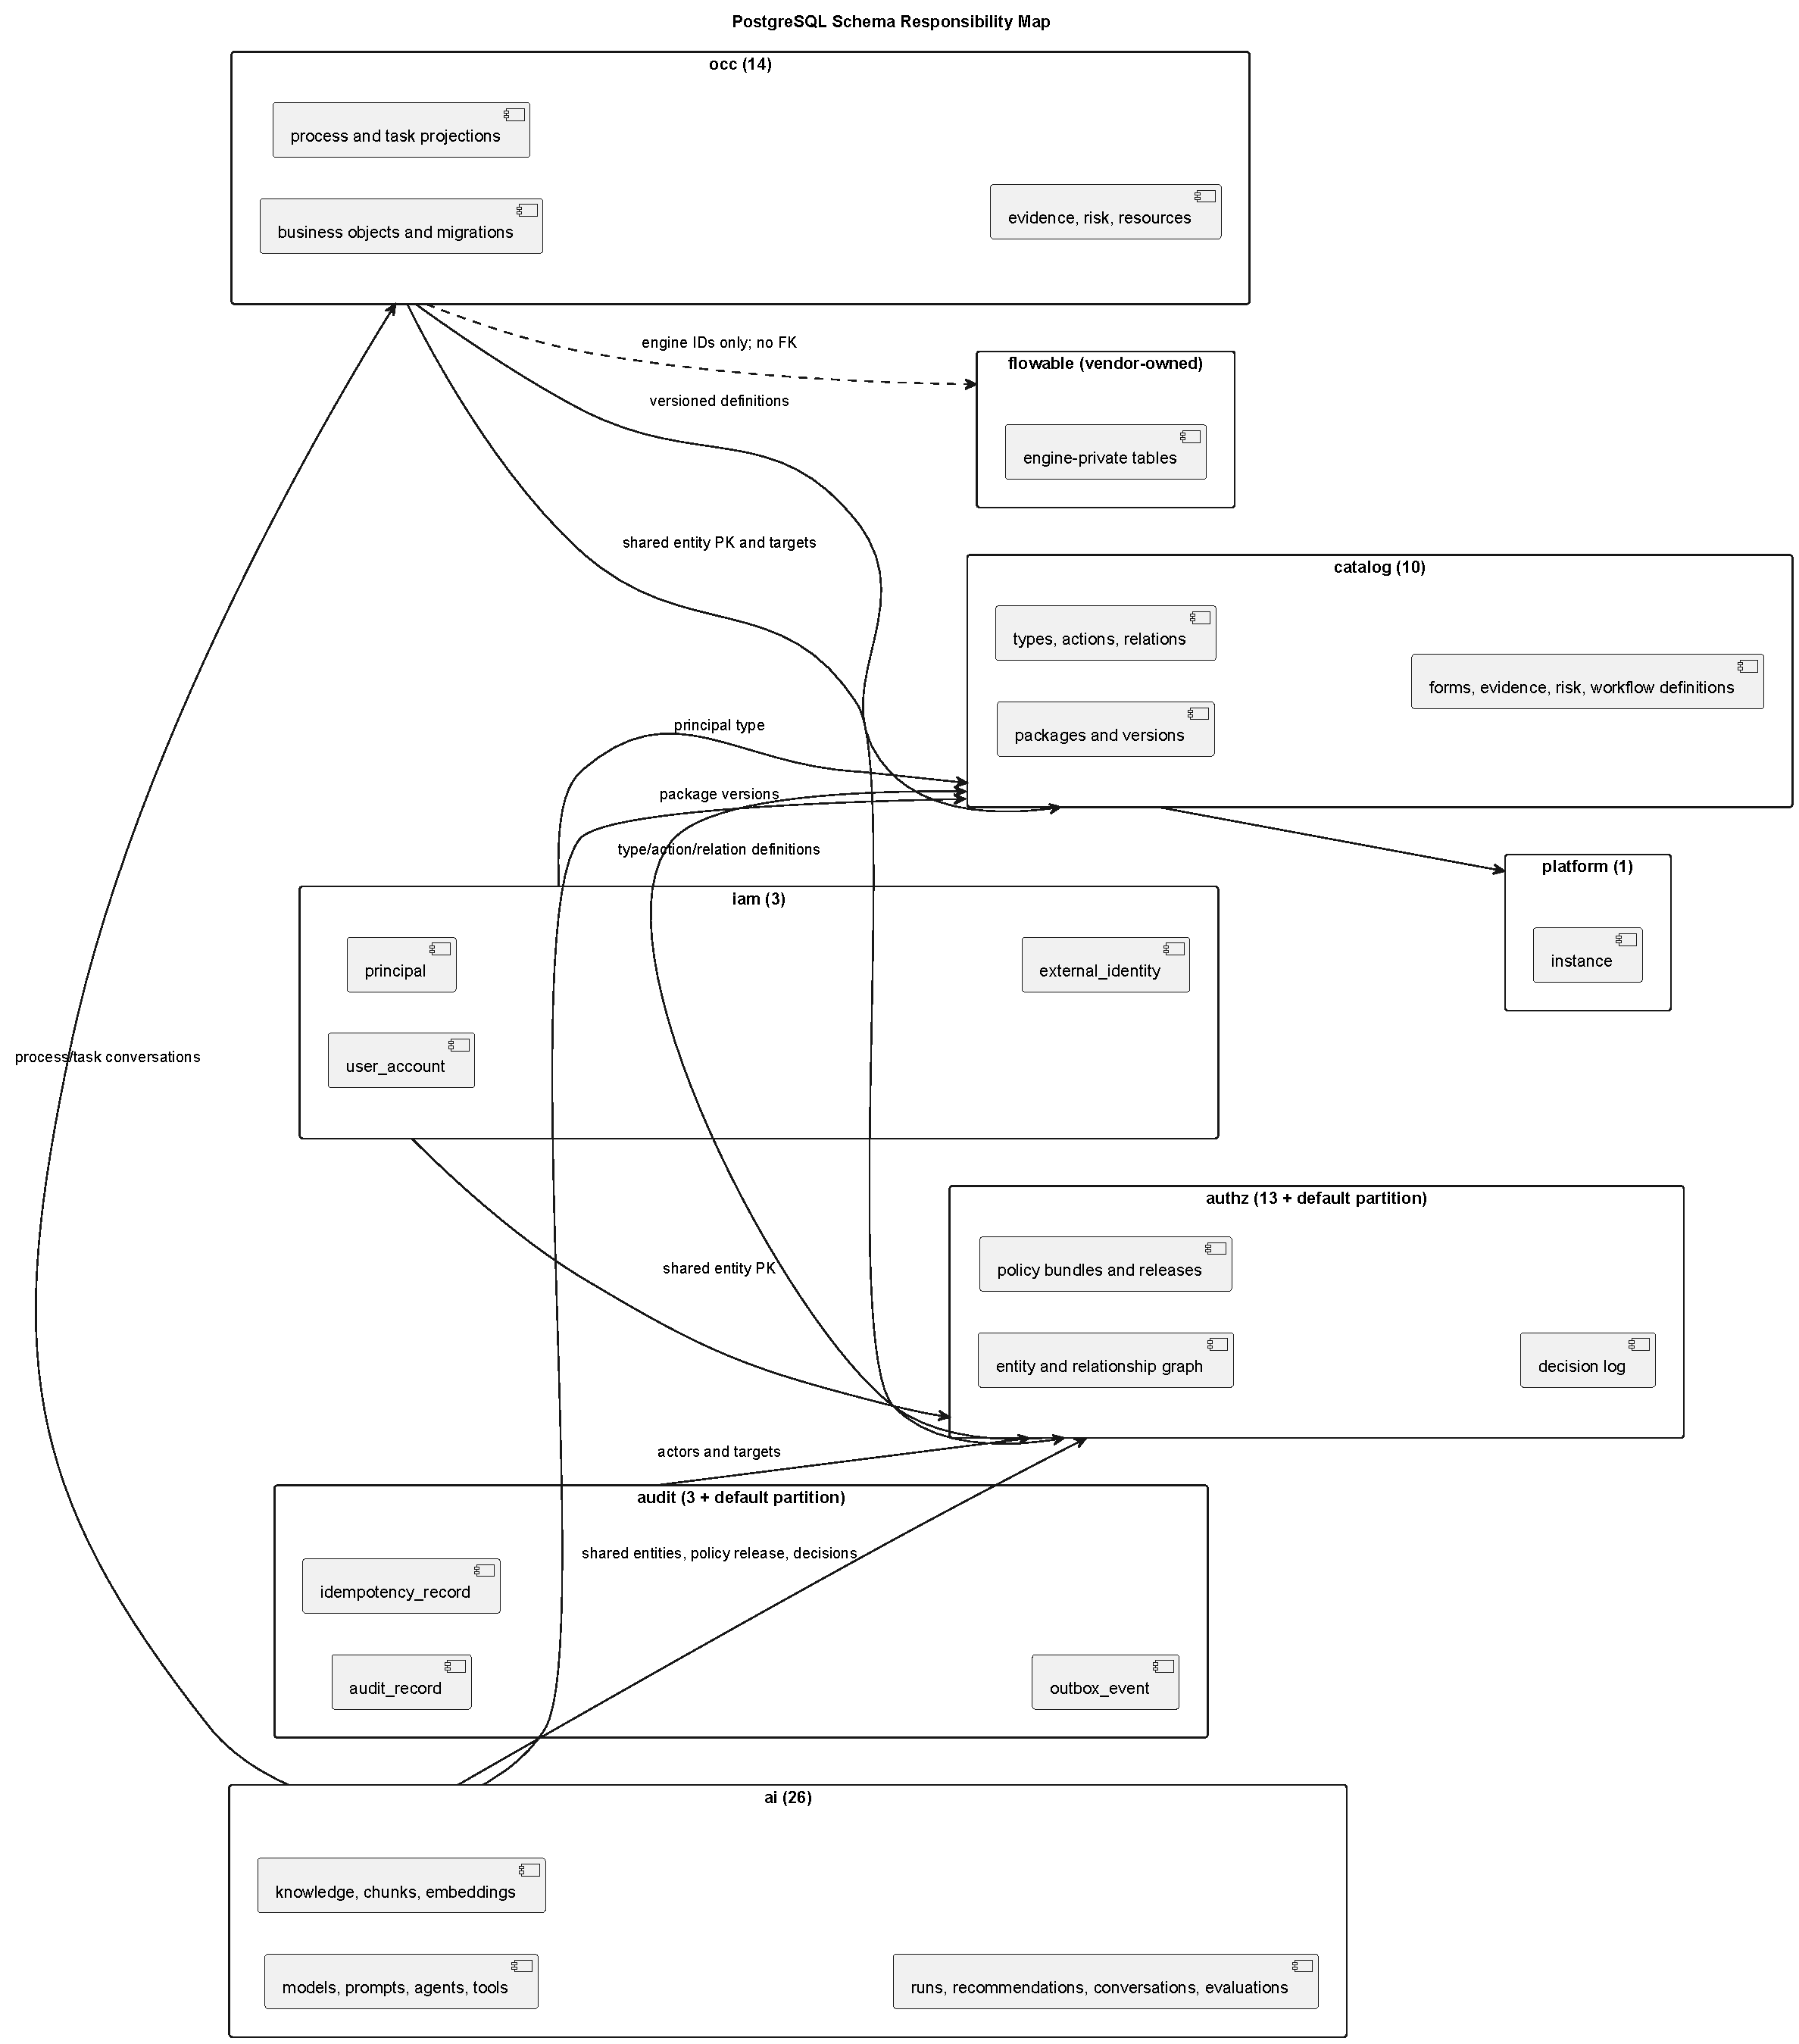
\includegraphics[width=\textwidth]{08-database-schema-map.pdf}
\caption{数据库 schema 职责和依赖方向。}
\label{fig:schemas}
\end{figure}

\subsection{通用约定}
标识使用应用生成 UUIDv7，时间为 UTC \texttt{timestamptz}，成本为 \texttt{numeric}，可扩展状态使用 text + CHECK。JSON 对象使用 \texttt{platform.is\_json\_object}。可变聚合以 \texttt{row\_version} 乐观锁，更新触发器同步 \texttt{updated\_at} 并递增版本。默认删除策略为 RESTRICT；草稿子项、索引投影和运行从属项才允许 CASCADE。

\subsection{Schema 与表清单}
\begin{longtable}{p{0.12\textwidth}p{0.08\textwidth}p{0.72\textwidth}}
\toprule
Schema & 数量 & 表 \\
\midrule
\endhead
platform & 1 & instance\\
catalog & 10 & domain\_package, package\_version, entity\_type, entity\_type\_version, action\_definition, relation\_definition, form\_definition, evidence\_requirement, risk\_rule\_definition, workflow\_definition\\
iam & 3 & principal, user\_account, external\_identity\\
authz & 13 & entity, authorization\_state, relationship, relationship\_closure, policy\_bundle, policy\_bundle\_version, policy\_module, policy\_test\_case, policy\_approval, policy\_binding, policy\_release, policy\_release\_item, decision\_log（另有 decision\_log\_default）\\
occ & 14 & business\_object, object\_index\_value, data\_migration, data\_migration\_item, process\_definition\_binding, process\_instance, task\_projection, upload\_session, evidence, evidence\_version, evidence\_review, risk, managed\_resource, resource\_reservation\\
audit & 3 & audit\_record, idempotency\_record, outbox\_event（另有 audit\_record\_default）\\
ai & 26 & model\_provider, model\_profile, prompt\_template, prompt\_template\_version, agent\_definition, agent\_definition\_version, tool\_definition, agent\_tool\_grant, knowledge\_source, knowledge\_document, knowledge\_document\_version, knowledge\_chunk, embedding\_space, chunk\_embedding, ai\_run, ai\_run\_artifact, tool\_call, recommendation, recommendation\_citation, conversation, message, evaluation\_dataset, evaluation\_dataset\_version, evaluation\_case, evaluation\_run, evaluation\_result\\
flowable & 0 & 供应商私有表由 Flowable 管理；OCC 只保存引擎 ID，不建立跨边界 FK。\\
\bottomrule
\end{longtable}

\subsection{统一实体与共享主键}
\texttt{authz.entity} 是授权超类型。\texttt{iam.principal}，六个 OCC 实体（business object、process instance、task、evidence、risk、managed resource）以及五个 AI 实体（provider、knowledge source/document、recommendation、conversation）与其共享主键。实体类型和类型版本使用组合 FK 保持一致；business object 进一步用组合 FK保证自身版本与授权实体一致。关系事实只保存在 \texttt{authz.relationship}，closure 是可重建查询投影，不能作为最终 ALLOW 依据。

\begin{figure}[H]
\centering
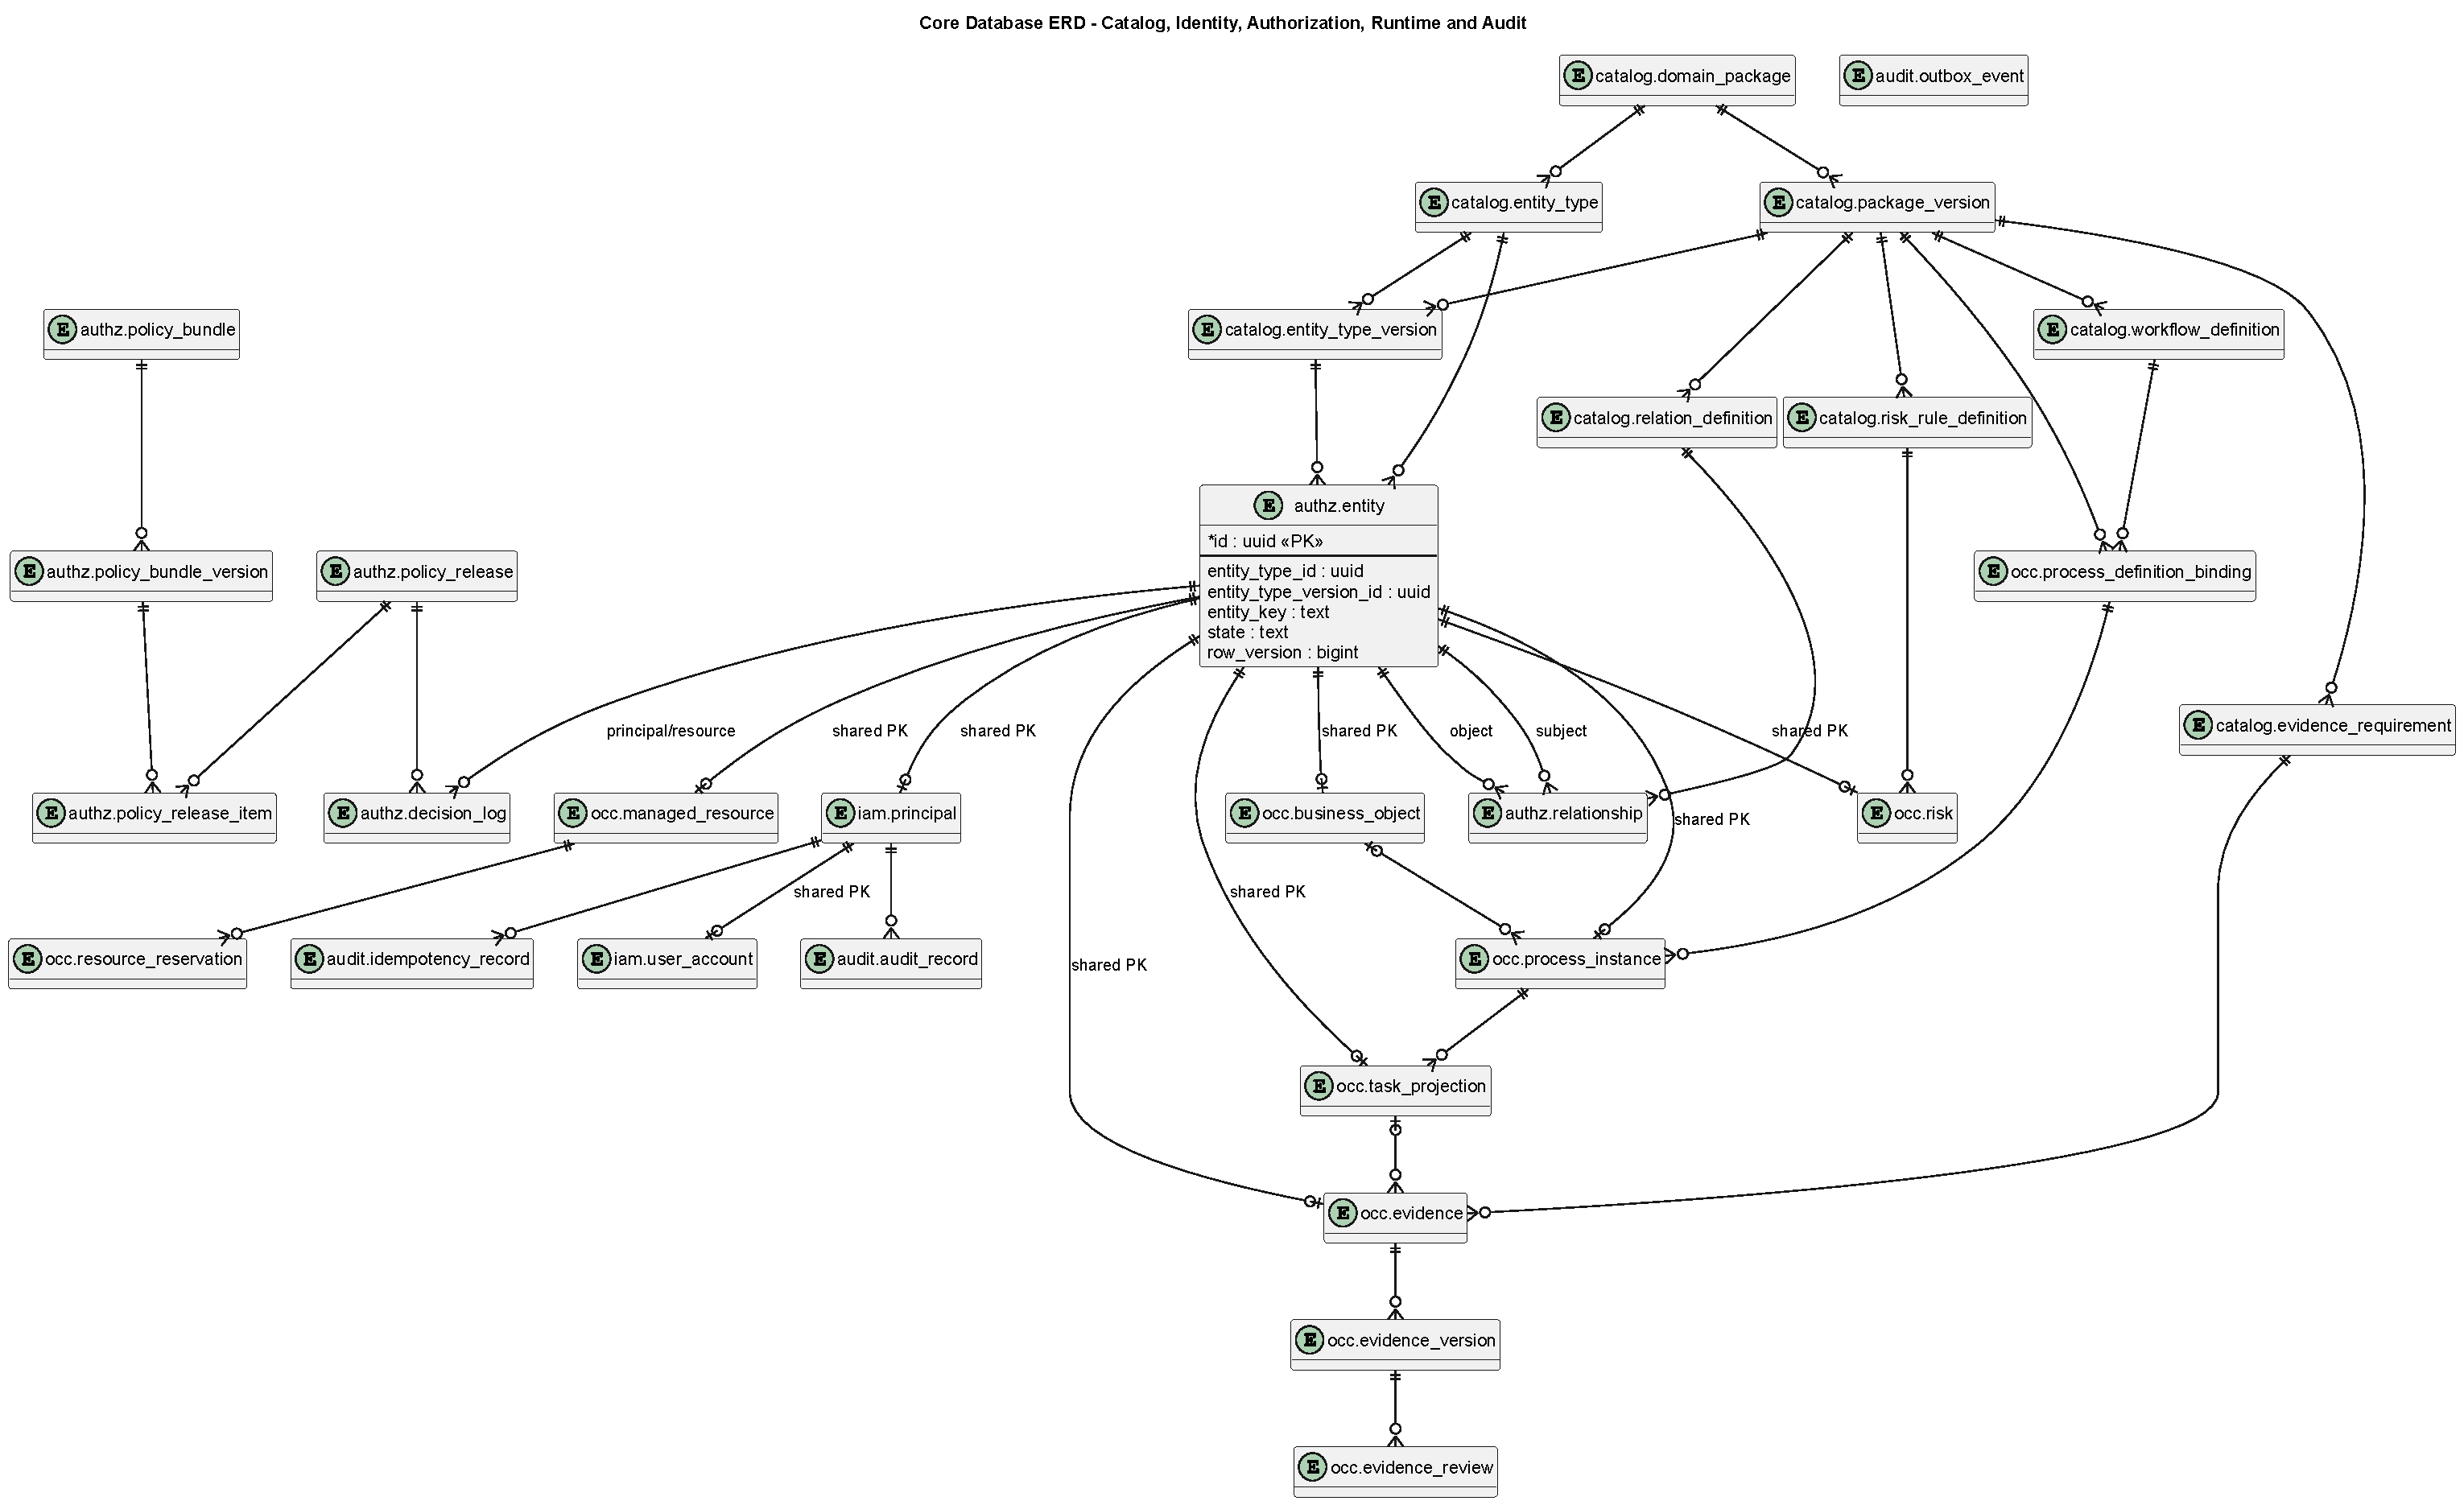
\includegraphics[width=\textwidth]{09-core-database-erd.pdf}
\caption{核心数据库 ER 图；为可读性省略部分字段和定义子表。}
\label{fig:coreerd}
\end{figure}

\subsection{可扩展业务数据}
\texttt{occ.business\_object.data} 保存经 JSON Schema 校验的领域字段，并永久绑定创建时的 entity type version。\texttt{object\_index\_value} 是 TEXT/NUMBER/TIMESTAMP/BOOLEAN 类型化可重建投影，不是 EAV 事实源。升级通过 data migration 与 item 显式追踪，单对象成功后才切换版本；失败可暂停重试。

\subsection{流程、证据与资源完整性}
Flowable deployment/definition/instance/task ID 均设唯一约束，但不对供应商表建立 FK。证据版本以对象 key、SHA-256、类型和大小形成不可变链；current version 通过可延迟组合 FK 指向本证据的版本。排他资源预约使用 GiST exclusion constraint 阻止重叠，容量总和由 Core 在锁定资源行的事务内校验。

\subsection{AI 与 RAG 数据模型}
\begin{figure}[H]
\centering
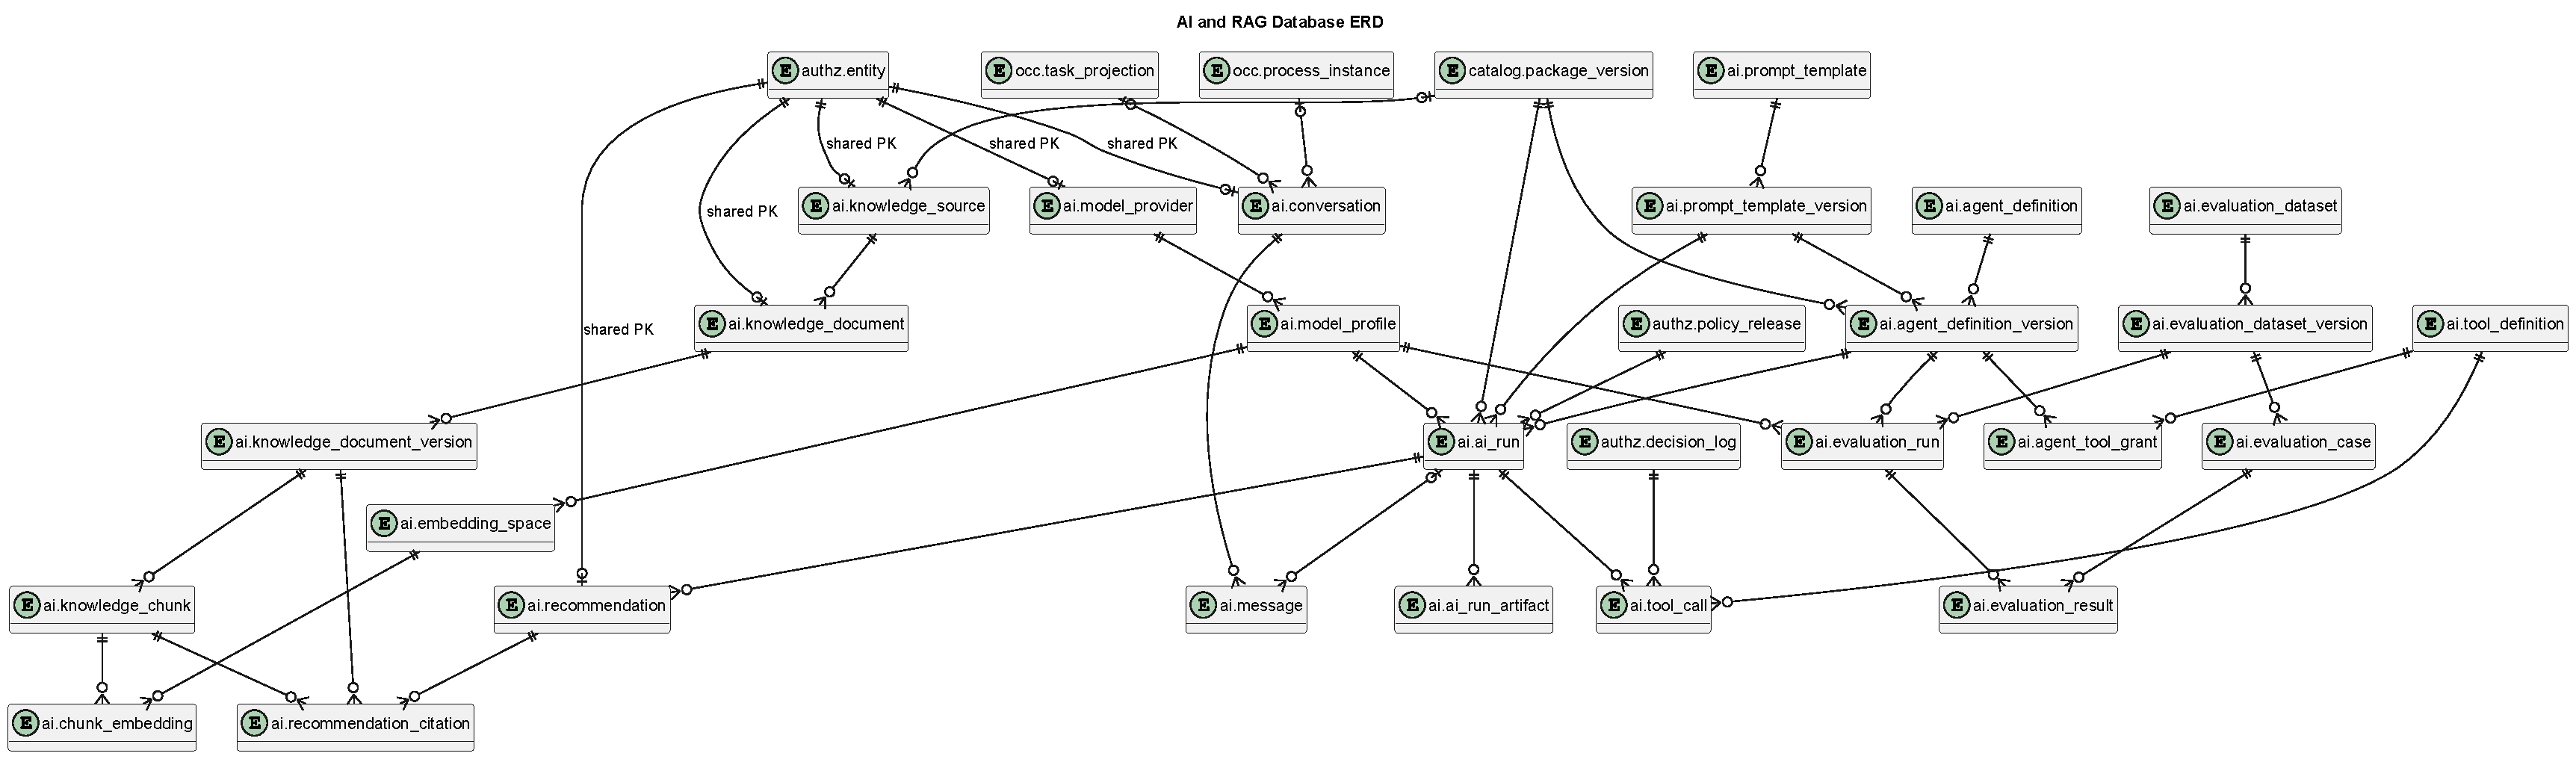
\includegraphics[width=\textwidth]{10-ai-database-erd.pdf}
\caption{AI、RAG、建议、会话与评测 ER 图。}
\label{fig:aierd}
\end{figure}
知识源和文档是授权实体，chunk 继承文档权限。全文索引使用生成的 \texttt{tsvector} 和 GIN；向量存储按 embedding space 列表分区，辅助函数为每个空间创建维度 CHECK 与 COSINE/L2/INNER PRODUCT 对应 HNSW 索引。tool call 通过 (decision log ID, created\_at) 组合 FK 关联分区决策日志。recommendation citation 组合 FK 保证 chunk 属于声明的 document version。

\subsection{索引、分区与不可变性}
主要索引覆盖实体类型/状态、关系双向遍历及有效期、JSONB business data、四种索引投影值、任务/证据/风险查询、待发布 Outbox、知识全文、AI run 和消息时间线。decision log 与 audit record 按时间范围分区并提供默认分区；chunk embedding 按空间列表分区。生产运维必须提前创建月分区并迁出默认分区数据。

\subsection{数据库账号边界}
目标设计至少包含迁移、Core、AI 和只读审计账号。AI 账号不得读取 Flowable、IAM 凭据或 OCC 私有表，也不得写 authz/iam/OCC；但当前迁移尚未创建角色、GRANT、受限视图或 RLS，因此这是部署脚本必须补齐的\statusgate。

\begin{figure}[H]
\centering
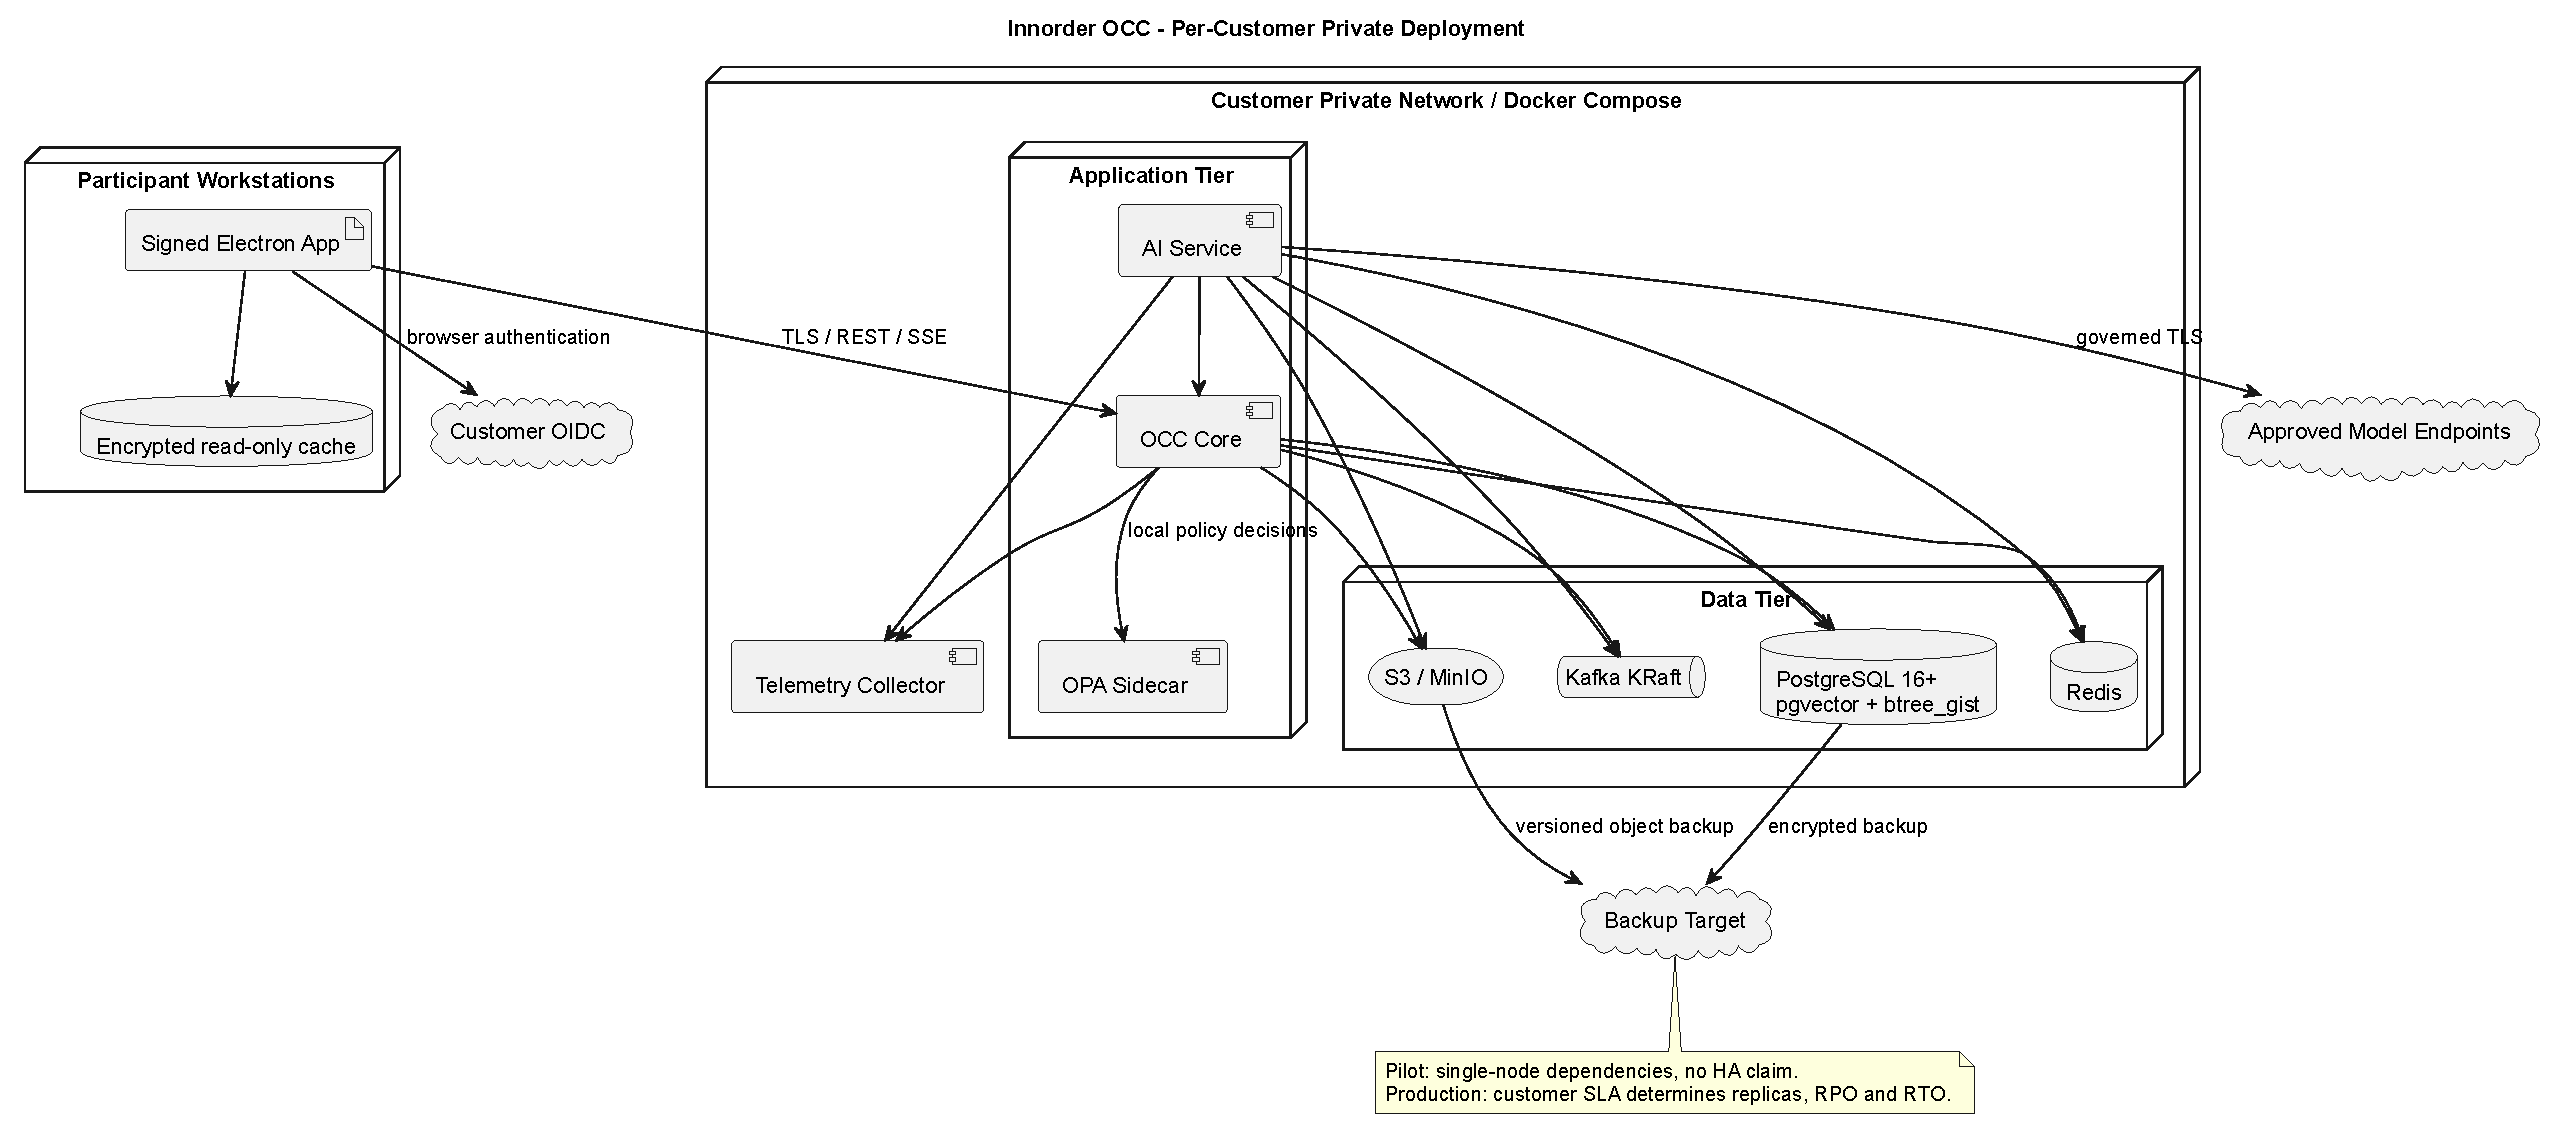
\includegraphics[width=0.95\textwidth]{07-deployment.pdf}
\caption{每客户独立私有部署拓扑。}
\label{fig:deployment}
\end{figure}

\section{验证与验收}
\subsection{现有验证证据}
静态 Node 测试检查八个迁移顺序、禁止 TODO/TBD、schema/extension、关键表、授权与并发保护、触发器返回模式、跨表版本和不可变策略内容。SQL 契约测试覆盖关键对象与若干变更约束。README 记录 PGlite 0.5.4 空库执行成功，但以兼容 domain 替代 pgvector。

\subsection{发布质量门禁}
\begin{enumerate}[leftmargin=*]
\item 在真实 PostgreSQL 16 + pgvector 从空库运行 V001--V008，并运行全部 SQL 契约测试。
\item 调用 \texttt{ai.create\_embedding\_partition}，验证维度约束、运算符类与 HNSW 索引。
\item 用 Testcontainers 验证 Flowable/OCC/audit/Outbox 原子事务、Kafka 重投、Redis 降级和对象上传。
\item 执行撤权、策略切换、关系变化与业务写并发测试，证明无 TOCTOU 越权。
\item 验证默认拒绝、DENY 优先、平台 DENY 不可覆盖、关系图基数与环检测。
\item 验证未授权文档不会进入 RAG 候选集合，并执行提示注入、工具越权和无来源输出测试。
\item 执行 Electron 安全、端到端、离线只读和安装签名测试。
\item 使用 k6 验证性能基线，演练备份恢复、策略回滚、分区归档和对象清理。
\end{enumerate}

\subsection{业务验收指标}
首轮 10--20 名学生试点目标：关键节点证据完整率 $\geq95\%$；违规跳步拦截率 $\geq90\%$；教师重复催办时间下降 $\geq30\%$；等待期高价值任务覆盖率 $\geq70\%$；已知严重红色风险漏报为 0；风险误报率 $\leq20\%$；学生周活跃率 $\geq80\%$；流程修改生效时间不超过一个工作日。

\section{实现差距与决策记录}
\begin{longtable}{p{0.29\textwidth}p{0.30\textwidth}p{0.33\textwidth}}
\toprule
主题 & 当前事实 & 处置要求 \\
\midrule
\endhead
服务账号凭据 & 设计称 USER/SERVICE 可认证，DDL 只有 USER-only user\_account。 & 实现前决定服务身份使用 OIDC client credential、mTLS 或新增受控表。\\
AI 运行不可变 & 设计称 AI run 只追加，DDL 未给 run/artifact/tool call/evaluation 添加不可变触发器。 & 明确状态机允许更新列，并在终态冻结或补充历史表。\\
月分区 & DDL 只有 audit/decision 默认分区，无月分区维护函数；AI run 未分区。 & 增加运维迁移与监控，按容量决定 AI 日志分区。\\
数据库最小权限 & DDL 未创建角色、GRANT 或受限视图。 & 作为部署交付物实现并做权限回归测试。\\
共享主键子类型 & principal 与 business object 有类型校验；其他共享 PK 实体未证明预期子类型。 & 在 Core 工厂或数据库 trigger 中补强并测试。\\
跨包一致性 & 若干 workflow/binding/instance 和 agent/prompt/package 对未完整校验同包兼容。 & 发布校验必须拒绝跨版本不一致引用，必要时增加组合 FK。\\
策略发布门禁 & DDL 不强制所有测试通过和审批完成。 & Core 发布命令必须检查编译、测试和审批结果，再改变状态。\\
真实 pgvector & PGlite 验证使用兼容类型，未验证真实 HNSW。 & 生产前门禁，不能以静态测试替代。\\
\bottomrule
\end{longtable}

\section{项目文档总结}
企划书给出了产品判断：首个场景选择嵌入式开发教学，以“人--任务--证据--资源--风险”为核心，在低责任、可重复环境验证控制内核，并以 16 周完成 10--20 人试点。技术架构文档把该愿景收敛为每客户私有部署、Electron 全员客户端、Flowable 嵌入式模块化 Core、独立 AI Service、OPA 三层授权、Kafka Outbox 事件和 Redis 可重建缓存。数据库设计进一步把跨领域能力落实为版本化 catalog、统一授权实体、JSONB 强类型核心、流程投影、不可变证据、显式数据迁移和授权优先的 RAG。SQL 迁移实现了上述大部分数据骨架与关键完整性，但应用服务、部署权限、真实基础设施集成和若干治理门禁仍待实现与验证。

\section{结论}
创序 OCC 的关键工程判断是把业务正确性放在确定性 Core 和事务数据库中，把 AI 限制为可追踪、可拒绝、可人工复核的建议系统。当前数据库基线足以支持领域包、授权图、流程投影、证据、风险、资源、Outbox 和 AI/RAG 的 MVP 开发；下一阶段应优先完成 Flowable 原子事务原型、OPA revision 并发验证、数据库账号隔离、真实 pgvector 测试和首条教学领域包，而不是扩展更多 Agent 或行业。

\begin{thebibliography}{9}
\bibitem{proposal} 创序 OCC 项目企划书，V1.0，2026-07。
\bibitem{architecture} 创序 OCC 技术选型与架构设计，2026-07-28。
\bibitem{database} 创序 OCC 数据库表设计，2026-07-28。
\bibitem{postgres} PostgreSQL Global Development Group, ``PostgreSQL Documentation,'' \url{https://www.postgresql.org/docs/}.
\bibitem{flowable} Flowable, ``Flowable Open Source Documentation,'' \url{https://www.flowable.com/open-source/docs/}.
\bibitem{opa} Open Policy Agent, ``OPA Documentation,'' \url{https://www.openpolicyagent.org/docs/latest/}.
\bibitem{pgvector} pgvector, ``Open-source vector similarity search for Postgres,'' \url{https://github.com/pgvector/pgvector}.
\end{thebibliography}

\end{document}
